\documentclass{report}
\setlength{\parskip}{\baselineskip}%
\usepackage{amsmath}
\usepackage{amsfonts,stmaryrd,amssymb} % Math packages

\usepackage{enumerate} % Custom item numbers for enumerations
\usepackage{fontawesome}
\usepackage{setspace}
\usepackage{hyperref}
\usepackage{enumitem}
\usepackage{multicol}
\usepackage{xhfill}
\usepackage[p,osf]{cochineal}
\usepackage[scale=.95,type1]{cabin}
\usepackage[cochineal,bigdelims,cmintegrals,vvarbb]{newtxmath}
\usepackage[zerostyle=c,scaled=.94]{newtxtt}
\usepackage[cal=boondoxo]{mathalfa}
\usepackage[export]{adjustbox}
\usepackage{vwcol}  
\usepackage{fancyhdr}
\DeclareSymbolFont{yhlargesymbols}{OMX}{yhex}{m}{n}
\DeclareMathAccent{\wideparen}{\mathord}{yhlargesymbols}{"F3}

\hypersetup{
	colorlinks=false,
	linkcolor=black,
	filecolor=black,      
	urlcolor=black,
	pdftitle={Overleaf Example},
	pdfpagemode=FullScreen,
	urlbordercolor=white,
}

\urlstyle{same}


	
\newenvironment{cequation}{
	\makeatletter
	\setbool{@fleqn}{false}
	\makeatother
	\begin{equation*}
		}{\end{equation*}}
		
\newcommand{\sol}{\noindent\textbf{Solution:} }
%----------------------------------------------------------------------------------------

\newcommand{\exercise}[1]{%
	\subsection*{\faPencil\ \ Exercise #1\hspace{0.5em}\xrfill[0.175\baselineskip]{1pt}}
}

\newcommand{\practice}[1]{%
	\subsection*{\faFlag\ \ Practice #1\hspace{0.5em}\xrfill[0.175\baselineskip]{1pt}}
}

\newcommand{\revision}[1]{%
	\section*{\faGears\ \ Revision Exercise #1\hspace{0.5em}\xrfill[0.175\baselineskip]{1pt}}
}

\usepackage[ruled]{algorithm2e} % Algorithms

\usepackage[framemethod=tikz]{mdframed} % Allows defining custom boxed/framed environments

\usepackage{listings} % File listings, with syntax highlighting
\lstset{
	basicstyle=\ttfamily, % Typeset listings in monospace font
}

%----------------------------------------------------------------------------------------
%	DOCUMENT MARGINS
%----------------------------------------------------------------------------------------

\usepackage{geometry} % Required for adjusting page dimensions and margins

\geometry{
	paper=a4paper, % Paper size, change to letterpaper for US letter size
	top=2.5cm, % Top margin
	bottom=3cm, % Bottom margin
	left=2.5cm, % Left margin
	right=2.5cm, % Right margin
	headheight=14pt, % Header height
	footskip=1.5cm, % Space from the bottom margin to the baseline of the footer
	headsep=1.2cm, % Space from the top margin to the baseline of the header
	%showframe, % Uncomment to show how the type block is set on the page
}

%----------------------------------------------------------------------------------------
%	FONTS
%----------------------------------------------------------------------------------------

\usepackage[utf8]{inputenc} % Required for inputting international characters
\usepackage[T1]{fontenc} % Output font encoding for international characters

%----------------------------------------------------------------------------------------
%	COMMAND LINE ENVIRONMENT
%----------------------------------------------------------------------------------------

% Usage:
% \begin{commandline}
%	\begin{verbatim}
%		$ ls
%		
%		Applications	Desktop	...
%	\end{verbatim}
% \end{commandline}

\mdfdefinestyle{commandline}{
	leftmargin=10pt,
	rightmargin=10pt,
	innerleftmargin=15pt,
	middlelinecolor=black!50!white,
	middlelinewidth=2pt,
	frametitlerule=false,
	backgroundcolor=black!5!white,
	frametitle={Command Line},
	frametitlefont={\normalfont\sffamily\color{white}\hspace{-1em}},
	frametitlebackgroundcolor=black!50!white,
	nobreak,
}

% Define a custom environment for command-line snapshots
\newenvironment{commandline}{
	\medskip
	\begin{mdframed}[style=commandline]
		}{
	\end{mdframed}
	\medskip
}

%----------------------------------------------------------------------------------------
%	FILE CONTENTS ENVIRONMENT
%----------------------------------------------------------------------------------------

% Usage:
% \begin{file}[optional filename, defaults to "File"]
%	File contents, for example, with a listings environment
% \end{file}

\mdfdefinestyle{file}{
	innertopmargin=1.6\baselineskip,
	innerbottommargin=0.8\baselineskip,
	topline=false, bottomline=false,
	leftline=false, rightline=false,
	leftmargin=2cm,
	rightmargin=2cm,
	singleextra={%
		\draw[fill=black!10!white](P)++(0,-1.2em)rectangle(P-|O);
		\node[anchor=north west]
		at(P-|O){\ttfamily\mdfilename};
		%
		\def\l{3em}
		\draw(O-|P)++(-\l,0)--++(\l,\l)--(P)--(P-|O)--(O)--cycle;
		\draw(O-|P)++(-\l,0)--++(0,\l)--++(\l,0);
	},
	nobreak,
}

% Define a custom environment for file contents
\newenvironment{file}[1][File]{ % Set the default filename to "File"
	\medskip
	\newcommand{\mdfilename}{#1}
	\begin{mdframed}[style=file]
		}{
	\end{mdframed}
	\medskip
}

%----------------------------------------------------------------------------------------
%	NUMBERED QUESTIONS ENVIRONMENT
%----------------------------------------------------------------------------------------

% Usage:
% \begin{question}[optional title]
%	Question contents
% \end{question}

\mdfdefinestyle{question}{
	innertopmargin=1.2\baselineskip,
	innerbottommargin=0.8\baselineskip,
	roundcorner=5pt,
	nobreak,
	singleextra={%
		\draw(P-|O)node[xshift=1em,anchor=west,fill=white,draw,rounded corners=3pt]{%
			\faCaretRight\ \textbf{Example \theQuestion\questionTitle}};
	},
}

\newcounter{Question} % Stores the current question number that gets iterated with each new question

% Define a custom environment for numbered questions
\newenvironment{question}[1][\unskip]{
	\bigskip
	\stepcounter{Question}
	\newcommand{\questionTitle}{~#1}
	\begin{mdframed}[style=question]
		}{
	\end{mdframed}
	\medskip
}

%----------------------------------------------------------------------------------------
%	SOLUTIONS ENVIRONMENT
%----------------------------------------------------------------------------------------

% Usage:
% \begin{solution}
%	Solution contents
% \end{solution}

\mdfdefinestyle{solution}{
	innertopmargin=1.2\baselineskip,
	innerbottommargin=0.8\baselineskip,
	roundcorner=5pt,
	nobreak,
	singleextra={%
		\draw(P-|O)node[xshift=1em,anchor=west,fill=white,draw,rounded corners=5pt]{解};
	},
}

% Define a custom environment for solutions
\newenvironment{solution}{
	\begin{mdframed}[style=solution]
		}{
	\end{mdframed}
}

%----------------------------------------------------------------------------------------
%	WARNING TEXT ENVIRONMENT
%----------------------------------------------------------------------------------------

% Usage:
% \begin{warn}[optional title, defaults to "Warning:"]
%	Contents
% \end{warn}

\mdfdefinestyle{warning}{
	topline=false, bottomline=false,
	leftline=false, rightline=false,
	nobreak,
	singleextra={%
		\draw(P-|O)++(-0.5em,0)node(tmp1){};
		\draw(P-|O)++(0.5em,0)node(tmp2){};
		\fill[black,rotate around={45:(P-|O)}](tmp1)rectangle(tmp2);
		\node at(P-|O){\color{white}\scriptsize\bf !};
		\draw[very thick](P-|O)++(0,-1em)--(O);%--(O-|P);
	}
}

% Define a custom environment for warning text
\newenvironment{warn}[1][Warning:]{ % Set the default warning to "Warning:"
	\medskip
	\begin{mdframed}[style=warning]
		\noindent{\textbf{#1}}
		}{
	\end{mdframed}
	\vspace{-0.5cm}
}

%----------------------------------------------------------------------------------------
%	INFORMATION ENVIRONMENT
%----------------------------------------------------------------------------------------

% Usage:
% \begin{info}[optional title, defaults to "Info:"]
% 	contents
% 	\end{info}

\mdfdefinestyle{info}{%
	topline=false, bottomline=false,
	leftline=false, rightline=false,
	nobreak,
	singleextra={%
		\fill[black](P-|O)circle[radius=0.6em];
		\node at(P-|O){\color{white}\scriptsize\bf \faInfo};
		\draw[very thick](P-|O)++(0,-0.8em)--(O);%--(O-|P);
	}
}

% Define a custom environment for information
\newenvironment{info}[1][Info:]{ % Set the default title to "Info:"
	\medskip
	\begin{mdframed}[style=info]
		\noindent{\textbf{#1}}
		}{
	\end{mdframed}
	\vspace{-0.5cm}
	
}

\mdfdefinestyle{explore}{%
	topline=false, bottomline=false,
	leftline=false, rightline=false,
	nobreak,
	singleextra={%
		\fill[black](P-|O)circle[radius=0.6em];
		\node at(P-|O){\color{white}\scriptsize\bf \faFlask};
		\draw[very thick](P-|O)++(0,-0.8em)--(O);%--(O-|P);
	}
}

% Define a custom environment for warning text
\newenvironment{explore}[1][Exploration Activity:]{ % Set the default warning to "Warning:"
	\medskip
	\begin{mdframed}[style=explore]
		\noindent{\large\textbf{#1}}
		}{
	\end{mdframed}
	\vspace{-0.5cm}
}

\mdfdefinestyle{think}{%
	topline=false, bottomline=false,
	leftline=false, rightline=false,
	nobreak,
	singleextra={%
		\fill[black](P-|O)circle[radius=0.6em];
		\node at(P-|O){\color{white}\scriptsize\bf \faQuestion};
		\draw[very thick](P-|O)++(0,-0.8em)--(O);%--(O-|P);
	}
}

% Define a custom environment for warning text
\newenvironment{think}[1][Think about It:]{ % Set the default warning to "Warning:"
	\medskip
	\begin{mdframed}[style=think]
		\noindent{\large\textbf{#1}}
		}{
	\end{mdframed}
	\vspace{-0.5cm}
}



\usepackage{tabularx}
\usepackage{hlist}
\usepackage{tasks}
\usepackage{tabularray}
\usepackage{multirow}
\newcolumntype{Y}{>{\centering\arraybackslash}X}

\begin{document}
\pagestyle{fancy}
%... then configure it.
\fancyhead{} % clear all header fields
\fancyhead[RO,LE]{\thepage}
\fancyhead[LO,RE]{\leftmark}
\fancyfoot{} % clear all footer fields

\fancyfoot[LO,RE]{Dong Zong Addmath Textbook Senior 1 Volume II}
\fancyfoot[RO,RE]{\thepage}

\onehalfspacing
\setcounter{chapter}{8}

\chapter{Trigonometric Functions of Arbitrary Angles}

\section{Trigonometric Functions of Arbitrary Angles}

In Chapter 8, we extended the concept of angle by defining angle using ray rotation. Putting the direction and amount of rotation into consideration, we know that there are positive angles, negative angles, and zero angles (0°) of any size, collectively referred to as arbitrary angles. Next, we will discuss angles in a Cartesian coordinate system.

\subsection*{Angles and Quadrants}

In a plane, any angle can be moved so that the vertex of the angle coincides with the origin of the Cartesian coordinate system, and the initial side of the angle lies on the positive x-axis. With that, the quadrant to which the terminal side of the angle belongs determines which quadrant the angle is in (or to which quadrant the angle belongs). If the terminal side of the angle lies on the coordinate axes, then the angle does not belong to any quadrant. For example:
\vspace{-1em}
\begin{enumerate}[label=(\arabic*)]
    \item As shown in figure (a), $30^\circ$ and $390^\circ$ are both angles in the first quadrant.
    \item As shown in figure (b), $120^\circ$ and $-240^\circ$ are both angles in the second quadrant.
    \item As shown in figure (c), $-1$ rad and $(-2\pi + 1)$ rad are both angles in the fourth quadrant.
    \item As shown in figure (d), $\dfrac{3\pi}{2}$ rad and $-90^\circ$ do not belong to any quadrant.
\end{enumerate}

\begin{center}
    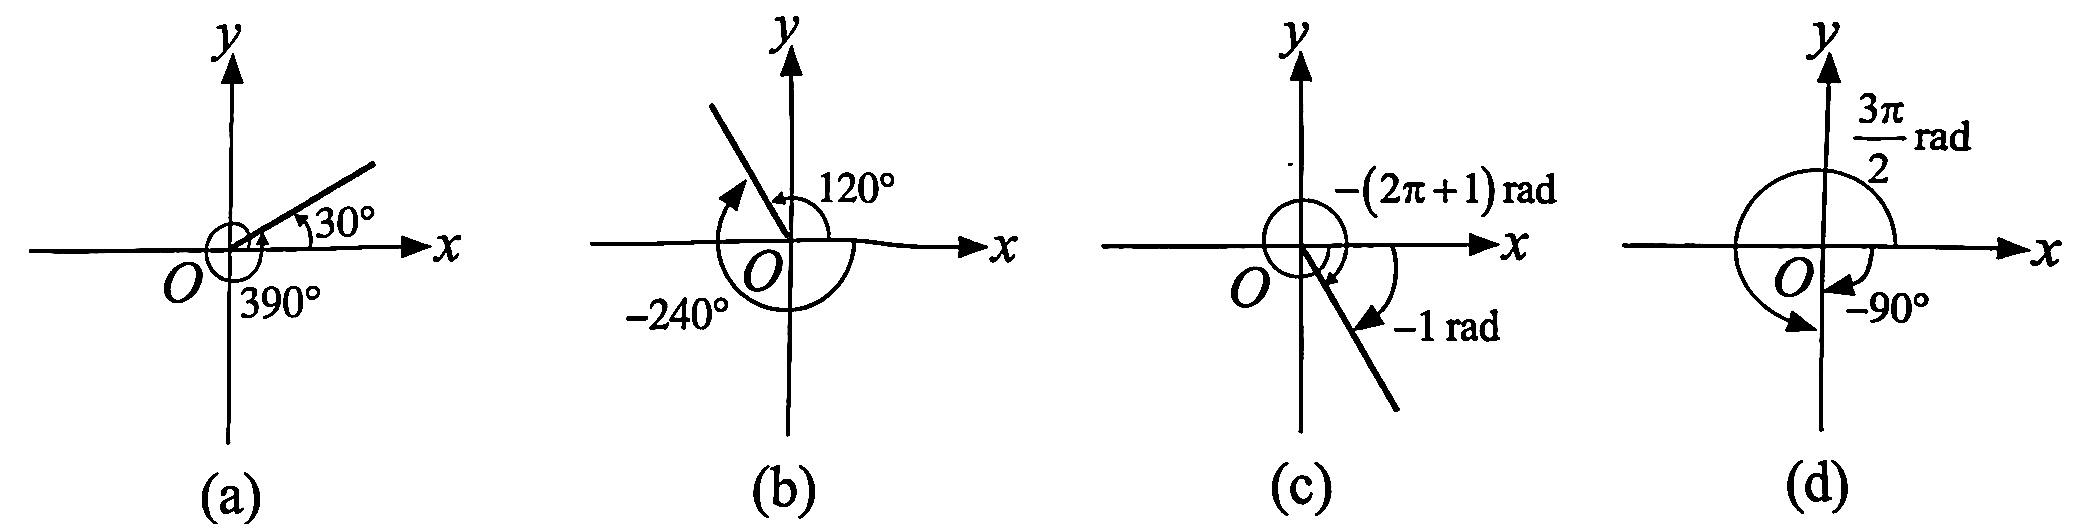
\includegraphics[width=0.8\textwidth]{assets/9-1.jpg}
\end{center}
\vspace{-1em}

\begin{think}
    Are "acute angle", "angle in the first quadrant", and "angle that is less than $90^\circ$" the same thing?
\end{think}

In this chapter, if not specified, the angles that we will discuss are angles of which the vertex is at the origin, and the initial side lies on the positive x-axis.

In the four sets of angles shown in the figures above, their initial and terminal sides are all the same. In fact, any angle $\theta$ that rotates one full round clockwise or counterclockwise will coincide with original terminal side, i.e. the terminal side of $\theta = 360^\circ$ or $\theta + (-360^\circ)$ will have the same terminal side as $\theta$. Using the same logic, we can conclude that: the angle $k \cdot 360^\circ + \circ$ will have the same terminal side as $\theta$ for $k \in \mathbb{Z}$.

\begin{question}
    Determine the quadrant to which the angle belongs.
    \vspace{-1em}
    \begin{multicols}{2}
        \begin{enumerate}[label=(\alph*)]
            \item $1020^\circ$
            \item $\dfrac{9}{4}\pi$
        \end{enumerate}
    \end{multicols}

    \sol{}
    \begin{multicols}{2}
        \begin{enumerate}[label=(\alph*)]
            \item $1020^\circ = 2(360^\circ) + 300^\circ$
                
            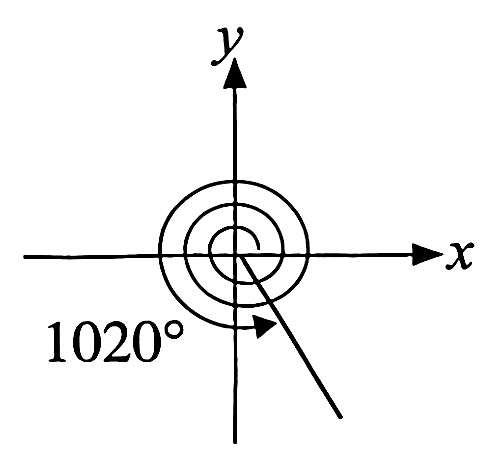
\includegraphics[width=0.2\textwidth]{assets/9-2.jpg}
            
            $\therefore 1020^\circ$ belongs to the fourth quadrant.
            \columnbreak

            \item $\dfrac{9}{4}\pi = 2\pi + \dfrac{\pi}{4}$
                
            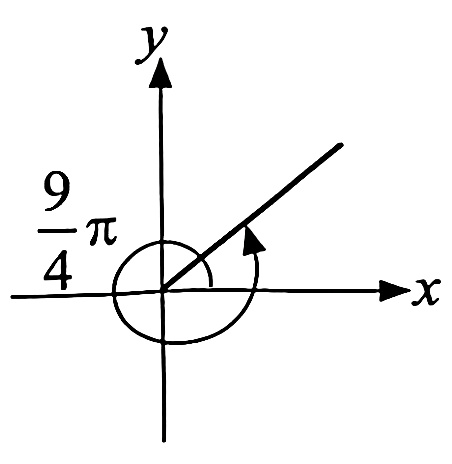
\includegraphics[width=0.2\textwidth]{assets/9-3.jpg}
            
            $\therefore \dfrac{9}{4}\pi$ belongs to the first quadrant.
        \end{enumerate}
    \end{multicols}
\end{question}

\practice{9.1a}
\begin{enumerate}
    \item Determine the quadrant to which the angle belongs.
    \begin{multicols}{4}
        \begin{enumerate}[label=(\alph*)]
            \item $\dfrac{2\pi}{3}$
            \item $740^\circ 50'$
            \item $-\dfrac{4\pi}{9}$
            \item $-135^\circ$
        \end{enumerate}
    \end{multicols}
    \item If $360^\circ < \theta < 450^\circ$, which quadrant does $\theta$ belong to?
    \item Given that $0^\circ < \theta < 360^\circ$ (i.e. $0 < \theta < 2\pi$), Find the angle $\theta$ with the same terminal side as the following angles:
    \begin{multicols}{4}
        \item $560^\circ 24'$
        \item $-15^\circ$
        \item $-1000^\circ$
        \item $\dfrac{12}{5}\pi$
    \end{multicols}
\end{enumerate}

\subsection*{Definition of Trigonometry Functions of Arbitrary Angles}

We have learned the trigonometric functions of acute angles: In a right triangle, the acute angle is the independent variable while the ratio of the sides is the value of the function.

Actually, now that we are discussing angles in a Cartesian coordinate system, we can also denote the trigonometric functions of the acute angles above in the form of coordinates. This definition can be further extended to situations where the angle is arbitrary.
\begin{center}
    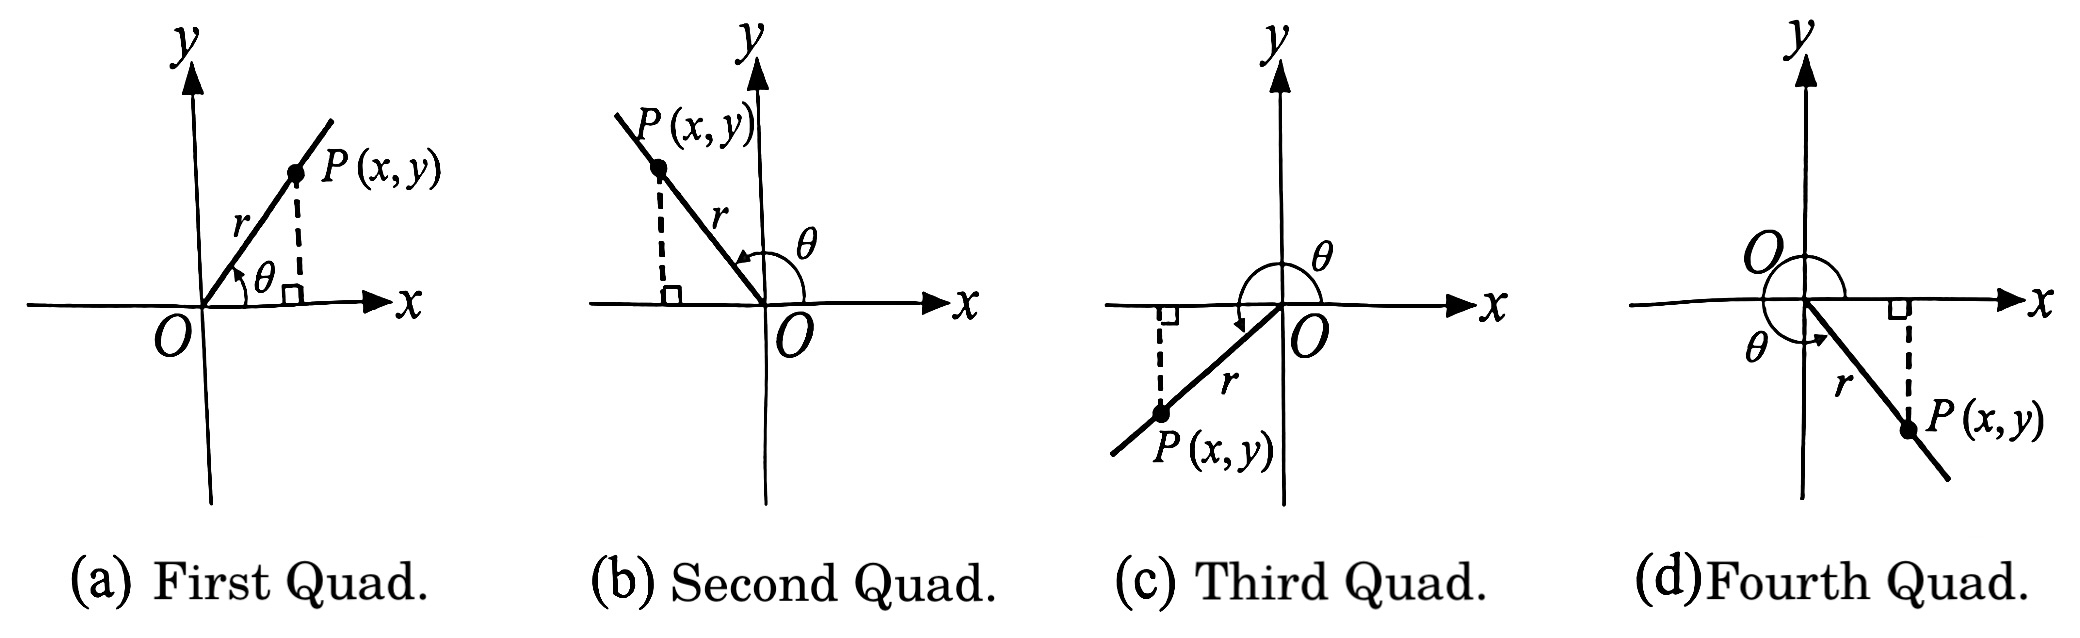
\includegraphics[width=0.8\textwidth]{assets/9-4.jpg}
\end{center}
\vspace{-1em}

As shown in the figure above, place an arbitrary angle $\theta$ in a coordinate system, and let the vertex of the angle as the origin, and the initial side of the angle lie on the positive x-axis. Take any point $P(x, y)$ on the terminal side of angle $\theta$ other than the origin, and let $r = OP = \sqrt{x^2 + y^2}$. Then, the trigonometric functions of angle $\theta$ are defined as follows:
\begin{info}[Trigonometric Functions of Arbitrary Angles]
    \begin{flalign*}
        \text{Sine} & \sin\theta = \dfrac{y}{r} & \text{Cosine} &\cos\theta = \dfrac{x}{r} &\\
        \text{Tangent} & \tan\theta = \dfrac{y}{x},\ x \neq 0 & \text{Cotangent} & \cot\theta = \dfrac{x}{y},\ y \neq 0 &\\
        \text{Secant} & \sec\theta = \dfrac{r}{x},\ x \neq 0 & \text{Cosecant} & \operatorname{cosec}\theta = \dfrac{r}{y},\ y \neq 0 &&&&&
    \end{flalign*}
\end{info}

\begin{question}
    Given that the terminal side of angle $\theta$ passes through point $P(2, -3)$, find the six trigonometric functions of angle $\theta$.

    \sol{}
    \vspace{-3em}
    \begin{multicols}{2}
        \begin{flalign*}
            \because\ &x=2, y=-3 &\\
            \therefore\ &r=\sqrt{2^2+(-3)^2} \\
            &\ \ =\sqrt{13} 
        \end{flalign*}
        \vspace{-3em}
        \begin{flalign*}
            \therefore\ \sin \theta&=\dfrac{y}{r}=\dfrac{-3}{\sqrt{13}}=-\dfrac{3 \sqrt{13}}{13} \\
            \cos \theta&=\dfrac{x}{r}=\dfrac{2}{\sqrt{13}}=\dfrac{2 \sqrt{13}}{13} \\
            \tan \theta&=\dfrac{y}{x}=\dfrac{-3}{2}=-\dfrac{3}{2} \\
            \cot \theta&=\dfrac{x}{y}=\dfrac{2}{-3}=-\dfrac{2}{3} \\
            \sec \theta&=\dfrac{r}{x}=\dfrac{\sqrt{13}}{2} \\
            \operatorname{cosec} \theta&=\dfrac{r}{y}=-\dfrac{\sqrt{13}}{3} &
        \end{flalign*}
        \vspace{1em}
            
        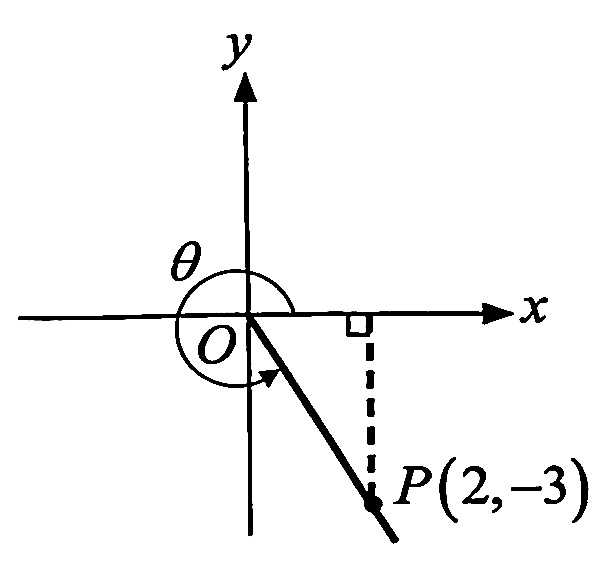
\includegraphics[width=0.24\textwidth]{assets/9-5.jpg}
    \end{multicols}
\end{question}
\begin{think}
    
    \noindent What is the relationship between the six trigonometric functions of an angle?
\end{think}

\practice{9.1b}

\vspace{-1em}
Given that $P\left(-\sqrt{3}, -1\right)$ is a point on the terminal side of angle $\alpha$, find the six trigonometric functions of angle $\alpha$.

\begin{explore}[Exploration Activity 1]
    
    \noindent \textbf{Definition of trigonometric functions in a unit circle}

    \noindent Given a circle with radius $r=1$ and center at the origin, take the intersection point $P(x, y)$ of the terminal side of angle $\theta$ with the circle. Since $r = OP = 1$, we have $\sin\theta = y$, $\cos\theta = x$, i.e. the vertical and horizontal coordinates of point $P$ are the sine and cosine of angle $\theta$ respectively.

    \noindent Now, open these GeoGebra Applet, inspect in action on how to define the sine function, cosine function, and tangent function using the coordinates of the point on the terminal side of $\theta$.

    \noindent \textbf{Tools:}
    \vspace{-1em}
    \begin{itemize}[leftmargin=*]
        \item Sine function and unit circle: \url{https://www.geogebra.org/m/xxjshdwq}
        \item Cosine function and unit circle: \url{https://www.geogebra.org/m/aajvmasj}
        \item Tangent function and unit circle: \url{https://www.geogebra.org/m/u6qg8x4z}
    \end{itemize}
\end{explore}

\vspace{-0.5em}
\subsection*{Trigonometric Values of Arbitrary Angles}

When defining the trigonometric functions of arbitrary angles, the initial side of the angle is fixed on the positive x-axis, and base on the size of $\theta$ and the direction of the rotation, the terminal side of the angle can be in any quadrant or on the coordinate axes. From this definition, we know that the value of the trigonometric functions of an angle is only determined by the location of the terminal side of the angle. Hence, $\theta$ and $\theta pm k \cdot 360^\circ$, $k \in \mathbb{Z}$ have the same value of trigonometric functions.

Regardless of the quadrant to which the terminal side of angle $\theta$ belongs, the value of $r$ is always positive ($r > 0$), while the value of $x$ and $y$ can be positive or negative, as shown in the table figure below. Hence, the trigonometric values of an angle can be positive or negative, depending on the quadrant to which the terminal side of the angle belongs, as shown in the table below.
\begin{vwcol}[widths={0.2,0.8}, sep=4mm, justify=flush, rule=0pt]
    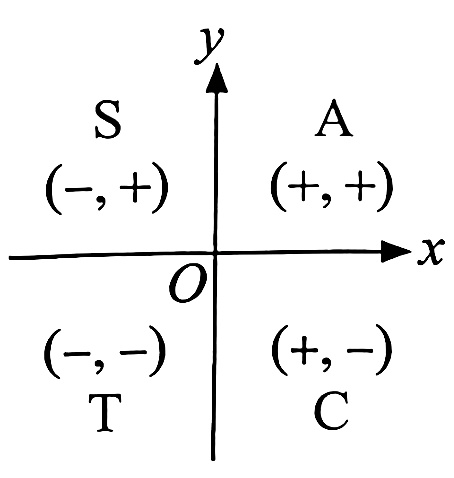
\includegraphics[width=0.2\linewidth]{assets/9-6.jpg}

    \parbox{0.8\textwidth}{\vspace{1.5em}\begin{tabular}{|c|c|c|c|c|}
        \hline  & First Quadrant & Second Quadrant & Third Quadrant & Fourth Quadrant \\
        \hline $\sin \theta$ & + & + & - & - \\
        \hline $\cos \theta$ & + & - & - & + \\
        \hline $\tan \theta$ & + & - & + & - \\
        \hline
        \end{tabular}}
\end{vwcol}
\begin{warn}[Note]
    
    \vspace{-1em} 
    \noindent $A$: All trigonometric values are positive

    \vspace{-1em}
    \noindent $S$: $\sin \theta$ is positive $\qquad$ $T$: $\tan \theta$ is positive $\qquad$ $C$: $\cos \theta$ is positive
    
    \vspace{-1em}
    \noindent The sign of the values of $\operatorname{cosec} \theta$, $\sec \theta$, and $\cot \theta$ are the same as the signs of $\sin \theta$, $\cos \theta$, and $\tan \theta$ respectively.
\end{warn}

\practice{9.1c}
\begin{enumerate}
    \item Without using a calculator, determine which quadrant the angle $\theta$ belongs to, and hence, find the sign of $\sin \theta$, $\cos \theta$, and $\tan \theta$:
    
    \begin{center}
        \begin{tabular}{|c|c|c|c|c|c|}
            \cline { 2 - 6 } \multicolumn{1}{c|}{} & $\theta$ & Quadrant & $\sin \theta$ & $\cos \theta$ & $\tan \theta$ \\
            \hline Example & $330^{\circ}$ & 4th & - & + & - \\
            \hline (a) & $-160^{\circ}$ & & & & \\
            \hline (b) & $210^{\circ}$ & & & & \\
            \hline (c) & $1068^{\circ}$ & & & & \\
            \hline (d) & $\dfrac{3 \pi}{4}$ & & & & \\
            \hline (e) & -5 & & & & \\
            \hline
            \end{tabular}
    \end{center}
    \item Base on the following conditions, determine which quadrant the angle $\theta$ belongs to:
    \begin{multicols}{2}
        \begin{enumerate}[label=(\alph*)]
            \item $\cot \theta<0$
            \item $\sin \theta>0$ and $\cos \theta<0$
            \item $\sec \theta<0$ and $\tan \theta>0$
            \item $\sin \theta \cdot \cot \theta>0$
        \end{enumerate}
    \end{multicols}
\end{enumerate}
\begin{question}
    Given that $\sin\theta = \dfrac{4}{5}$. Without finding the value of angle $\theta$, find the value of $\tan\theta$ and $\sec\theta$.

    \sol{}

    \noindent Given that $\sin\theta > 0$, hence $\theta$ belongs to the first or second quadrant. 

    \vspace{-1em}
    \begin{multicols}{2}
        \noindent Let $r = 5$, $y = 4$
        \vspace{-1em}
    \begin{enumerate}[label=(\roman*),leftmargin=*]
        \item If $\theta$ is in the first quadrant, then $x = \sqrt{5^2 - 4^2} = 3$,
        
        $\therefore$ $\tan\theta = \dfrac{4}{3}$, $\sec\theta = \dfrac{5}{3}$

        \item If $\theta$ is in the second quadrant, then $x = -\sqrt{5^2 - 4^2} = -3$,
        
        $\therefore$ $\tan\theta = -\dfrac{4}{3}$, $\sec\theta = -\dfrac{5}{3}$
    \end{enumerate}
    \vfill\null

    \begin{center}
        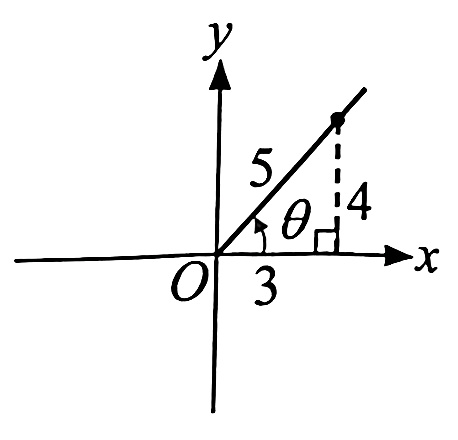
\includegraphics[width=0.2\textwidth]{assets/9-7.jpg}
    \end{center}
    \vspace{-3em}
    \begin{center}
        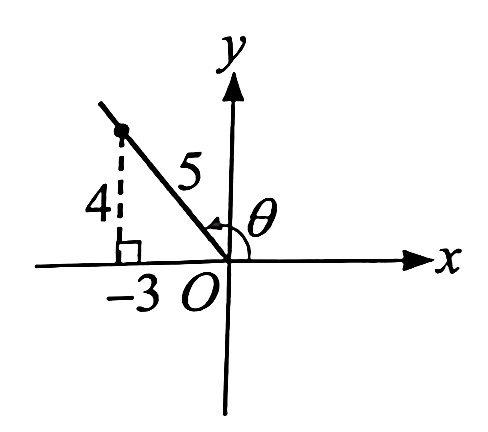
\includegraphics[width=0.21\textwidth]{assets/9-8.jpg}
    \end{center}
    \end{multicols}
\end{question}

\vspace{-1em}
In Example 3, we can see that there is an acute angle between the terminal side of $\theta$ and the $x$-axis.
\begin{center}
    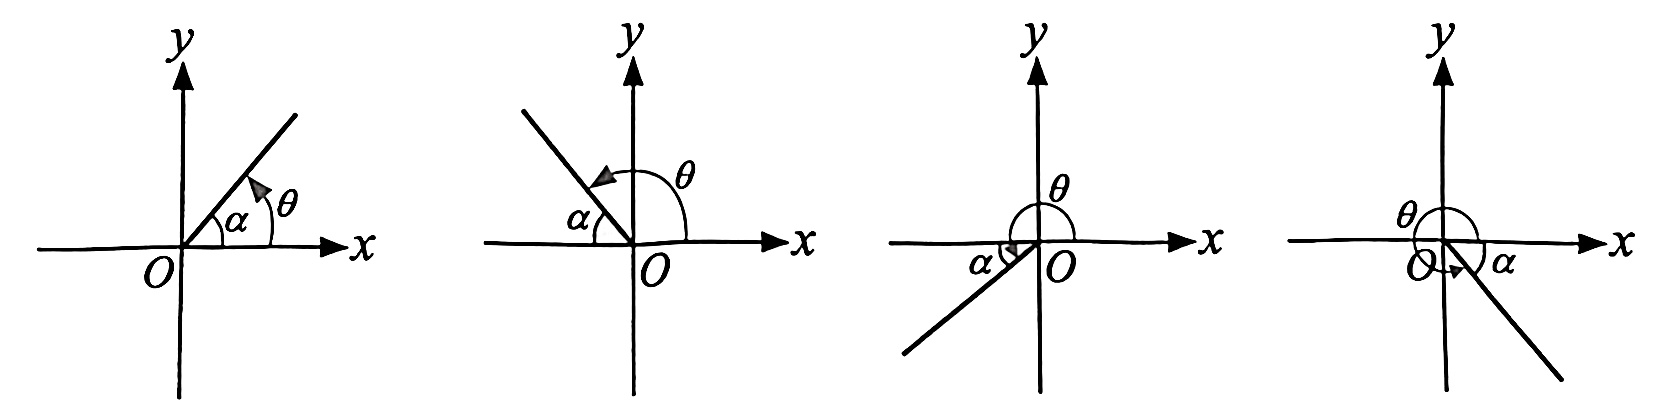
\includegraphics[width=0.8\textwidth]{assets/9-9.jpg}
\end{center}

As shown in the figure, no matter which quadrant $\theta$ belongs to, the acute angle $\alpha$ between its terminal side and the $x$-axis is known as the \textbf{associated acute angle} or \textbf{reference angle} of $\theta$. Since the acute angle $\alpha$ is in the first quadrant, the trigonometric values of $\alpha$ are always positive, and we can see that the absolute trigonometric values of $\theta$ is the same as the trigonometric values of $\alpha$. Hence, using the sign of the trigonometric functions and the trigonometric values of the reference angle, we can convert the problems of finding the trigonometric values of arbitrary angles to finding the trigonometric values of acute angles.

\begin{question}
    Convert the following expressions into trigonometric functions of acute angles:
    \vspace{-1em}
    \begin{multicols}{3}
        \begin{enumerate}[label=(\alph*)]
            \item $\sin 565^\circ$
            \item $\operatorname{cosec}\left(-285^\circ\right)$
            \item $\cos\dfrac{9\pi}{10}$
        \end{enumerate}
    \end{multicols}

    \sol{}
    \begin{enumerate}[label=(\alph*)]
        \item \begin{multicols}{2}
            $565^\circ$ is in the third quadrant, $\sin 565^\circ < 0$, the reference angle is $25^\circ$,

            $\therefore$ $\sin 565^\circ = -\sin 25^\circ$

            \vfill\null

            \begin{center}
                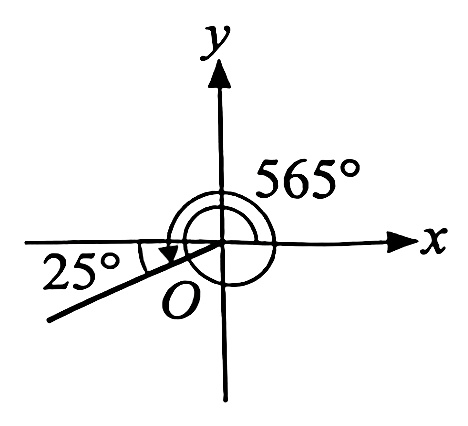
\includegraphics[width=0.2\textwidth]{assets/9-10.jpg}
            \end{center}
        \end{multicols}

        \item \begin{multicols}{2}
            $-285^\circ$ is in the first quadrant, $\operatorname{cosec}(-285^\circ) > 0$, the reference angle is $75^\circ$,

            $\therefore$ $\operatorname{cosec}(-285^\circ) = \operatorname{cosec}75^\circ$

            \vfill\null
            \begin{center}
                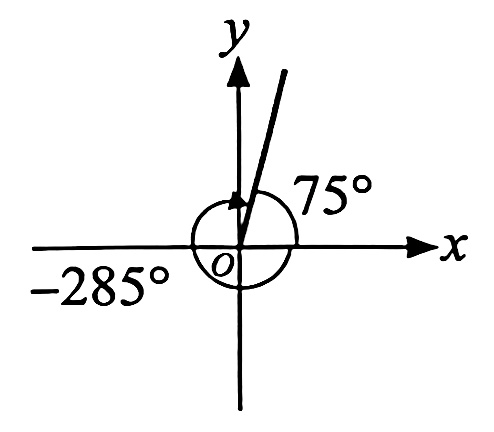
\includegraphics[width=0.2\textwidth]{assets/9-11.jpg}
            \end{center}
        \end{multicols}

        \item \begin{multicols}{2}
            $\dfrac{9\pi}{10}$ is in the second quadrant, $\cos\dfrac{9\pi}{10} < 0$, the reference angle is $\dfrac{\pi}{10}$,

            $\therefore$ $\cos\dfrac{9\pi}{10} = -\cos\dfrac{\pi}{10}$

            \vfill\null
            \begin{center}
                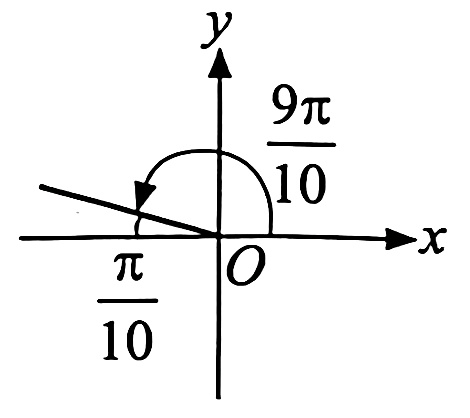
\includegraphics[width=0.2\textwidth]{assets/9-12.jpg}
            \end{center}
        \end{multicols}
    \end{enumerate}
\end{question}

\newpage
\begin{question}
    Without using a calculator, find the values of the following expressions:
    \begin{tasks}[label=(\alph*)](4)
        \task $\sin 300^\circ$
        \task $\tan\left(-150^\circ\right)$
        \task $\cot\left(\dfrac{17\pi}{4}\right)$
        \task $\cos^2 210^\circ$
    \end{tasks}

    \sol{}
    \vspace{-1em}
        \begin{enumerate}[label=(\alph*),leftmargin=*]
            \item \begin{multicols}{2}
                $\begin{aligned}[t]
                    \sin 300^\circ &= -\sin 60^\circ \\
                    &= -\dfrac{\sqrt{3}}{2}
                \end{aligned}$
                \vfill\null
                \begin{center}
                    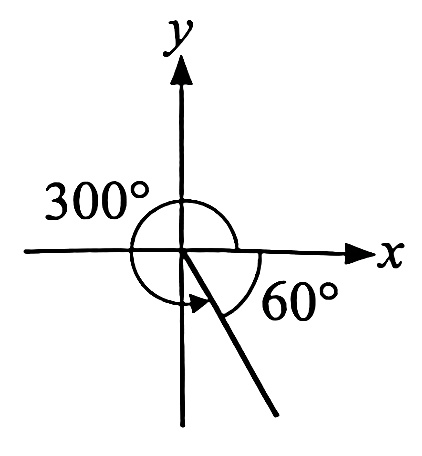
\includegraphics[width=0.2\textwidth]{assets/9-13.jpg}
                \end{center}
            \end{multicols}
            \vspace{-3.2em}
            \item \begin{multicols}{2}
                $\begin{aligned}[t]
                    \tan\left(-150^\circ\right) &= \tan 30^\circ \\
                    &= \dfrac{\sqrt{3}}{3}
                \end{aligned}$
                \vfill\null
                \begin{center}
                    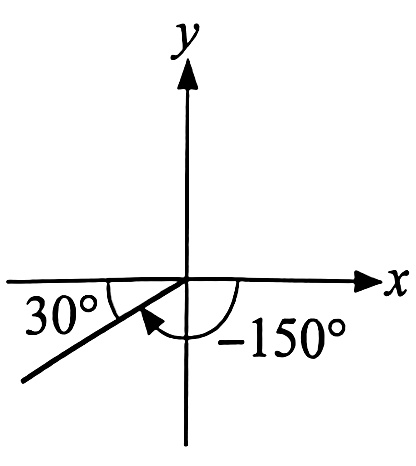
\includegraphics[width=0.2\textwidth]{assets/9-14.jpg}
                \end{center}
            \end{multicols}
            \vspace{-3.2em}
            \item \begin{multicols}{2}
                $\begin{aligned}[t]
                    \cot\left(\dfrac{17\pi}{4}\right) &= \cot\dfrac{\pi}{4} \\
                    &= 1
                \end{aligned}$
                \vfill\null
                \begin{center}
                    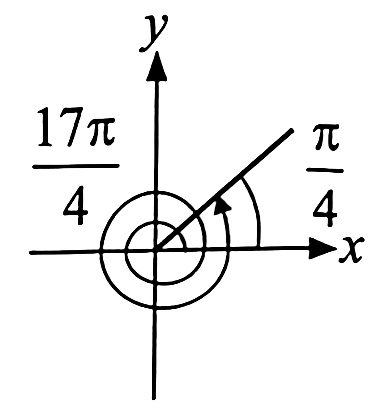
\includegraphics[width=0.2\textwidth]{assets/9-15.jpg}
                \end{center}
            \end{multicols}
            \vspace{-3.2em}
            \item \begin{multicols}{2}
                $\begin{aligned}[t]
                    \cos^2 210^\circ &= \cos^2 30^\circ \\
                    &= \dfrac{3}{4}
                \end{aligned}$
                \vfill\null
                \begin{center}
                    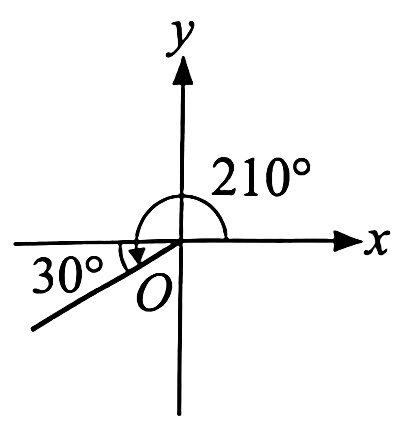
\includegraphics[width=0.2\textwidth]{assets/9-16.jpg}
                \end{center}
            \end{multicols}
        \end{enumerate}
\end{question}

\begin{question}
    \begin{multicols}{2}
        Given that $\cos\theta = \cos 50^\circ$, find the value of $\theta$.

    \sol{}

    \vspace{-0.5em}
    \noindent $\because$ $\cos 50^\circ > 0$, $\therefore$ $\theta$ is in the first or fourth quadrant.
    
    \vspace{-1em}
    \noindent $\because$ Reference angle is $50^\circ$,

    \vspace{-1em}
    \noindent $\therefore$ $\theta = 50^\circ$ or $\theta = 360^\circ - 50^\circ = 310^\circ$

    \begin{center}
        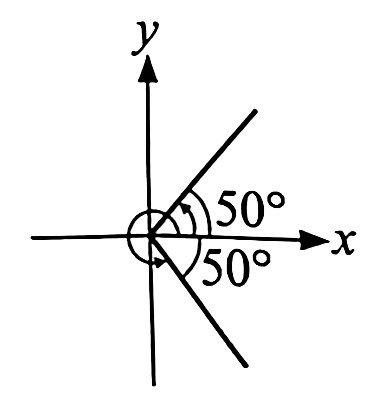
\includegraphics[width=0.2\textwidth]{assets/9-17.jpg}
    \end{center}
    \end{multicols}
\end{question}

\practice{9.1d}
\begin{enumerate}
    \item Let $180^\circ < A < 270^\circ$ and $\cot A = \dfrac{24}{7}$. Without finding the angle $A$, find the values of $\cos A$ and $\operatorname{cosec} A$.

    \item Without using a calculator, find the values of the following trigonometric functions:
    \begin{tasks}[label=(\alph*)](4)
        \task $\cos 150^\circ$
        \task $\sec (-330^\circ)$
        \task $\sin 690^\circ$
        \task \vspace*{-1.8em} $\cot \left(-\dfrac{5 \pi}{4}\right)$
    \end{tasks}

    \item Given $\sin \alpha = -\sin \dfrac{\pi}{8}$, and $0 \leq \alpha \leq 2 \pi$, find the value of $\alpha$.

\item \begin{enumerate}[label=(\alph*)]
\item Given $\sin 16^\circ \approx 0.2756$, find $\sin 164^\circ$.
\item Given $\cos 696^\circ \approx 0.9135$, find $\cos 24^\circ$.
\end{enumerate}
\end{enumerate}

\begin{vwcol}[widths={0.6,0.4}, sep=4mm, justify=flush, rule=0pt]
    We have previously discussed the signs of the trigonometric functions in different quadrants. In the next section, we will discuss the situations where the terminal side of the angle lies on the coordinate axes. Reviewing exploration activity 1, we can see that (as shown in the figure to the right):
    
    \noindent \parbox{0.58\textwidth}{\begin{enumerate}[label=(\roman*),leftmargin=*]
        \item When the terminal side of the angle lies on the $x$-axis, the $y$-coordinate of the intersection point $P$ is 0, hence, $\cot\theta$ and $\operatorname{cosec}\theta$ are undefined.
        \item When the terminal side of the angle lies on the $y$-axis, the $x$-coordinate of the intersection point $P$ is 0, hence, $\tan\theta$ and $\sec\theta$ are undefined.
    \end{enumerate}}
    
    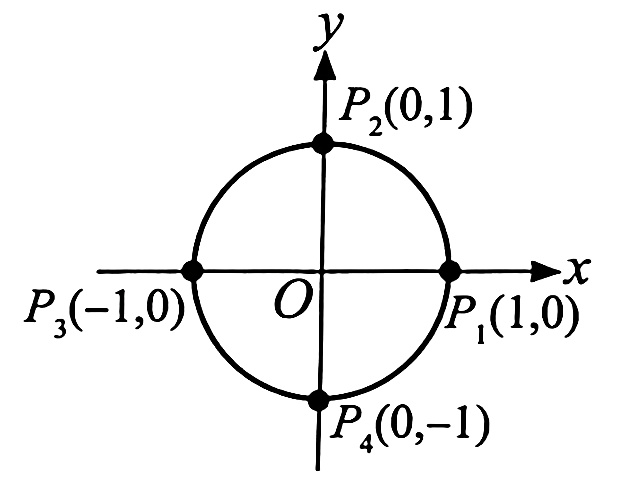
\includegraphics[width=0.34\linewidth]{assets/9-18.jpg}
\end{vwcol}
\vspace{-2em}
Listed in the following table are the sine, cosine, and tangent values of $0^\circ$, $90^\circ$, $180^\circ$, and $270^\circ$:
\begin{center}
    \begin{tabular}{|c|c|c|c|c|}
        \hline$\theta$ & $0^{\circ}$ & $90^{\circ}$ & $180^{\circ}$ & $270^{\circ}$ \\
        \hline $\sin \theta$ & 0 & 1 & 0 & -1 \\
        \hline $\cos \theta$ & 1 & 0 & -1 & 0 \\
         \hline $\tan \theta$ & 0 & undefined & 0 & undefined \\
        \hline
        \end{tabular}
\end{center}

\practice{9.1e}

Complete the following table:
\begin{center}
    \begin{tabularx}{0.8\textwidth}{|Y|Y|Y|Y|Y|}
        \hline$\theta$ & $0$ & $\dfrac{\pi}{2}$ & $\pi$ & $\dfrac{3 \pi}{2}$ \\
        \hline $\cot \theta$ & & & & \\
        \hline $\sec \theta$ & & & & \\
        \hline $\operatorname{cosec} \theta$ & & & & \\
        \hline
        \end{tabularx}
\end{center}

\newpage

\exercise{9.1}

\begin{enumerate}
    \item Determine in which quadrant the terminal side of each of the following angles lies:
    \begin{tasks}[label=(\alph*)](4)
        \task $840^\circ$
        \task $-190^\circ$
        \task \vspace*{-1.2em}$\dfrac{7 \pi}{4}$
        \task $-2$
    \end{tasks}

    \item Given that the terminal side of angle $\alpha$ passes through the following points, find the six trigonometric function values of $\alpha$:
    \begin{tasks}[label=(\alph*)](2)
        \task $(-8,-6)$
        \task $(-2,1)$
    \end{tasks}

    \item Without using a calculator, determine whether the following trigonometric values are positive or negative:
    \begin{tasks}[label=(\alph*)](4)
        \task $\cos 250^\circ$
        \task $\operatorname{cosec} \left(-1300^\circ\right)$
        \task $\tan 4$
        \task $\sin \left(-\dfrac{13}{3} \pi\right)$
    \end{tasks}

    \item Determine the quadrant to which angle $\theta$ belongs based on the following conditions:
    \begin{tasks}[label=(\alph*)](2)
            \task \vspace*{-2.4em}$\cos \theta = \dfrac{1}{3}$
            \task $\cos \theta$ and $\operatorname{cosec} \theta$ have the same sign
            \task $\dfrac{\sin \theta}{\cot \theta} < 0$
            \task \vspace*{-0.3em}$\tan^2 \theta = 3$
    \end{tasks}

    \item If $\sec \alpha = -\dfrac{17}{15}$, without finding the angle $\alpha$, find the values of $\sin \alpha$ and $\tan \alpha$.

    \item If $\sin \theta = k$, where $k < 0$ and $\cos \theta > 0$, express $\tan \theta$ in terms of $k$.
    
    \item Express the following trigonometric functions as acute angle trigonometric functions:
    \begin{tasks}[label=(\alph*)](4)
            \task $\operatorname{cosec} 186^\circ$
            \task $\cot \left(-505^\circ\right)$
            \task $\sin 7.6 \pi$
            \task $\cos \left(-\dfrac{59}{17} \pi\right)$
    \end{tasks}

    \item Given $0 \leq \theta \leq 360^\circ$, without using a calculator, find the value of $\theta$ in each of the following equations:
    \begin{tasks}[label=(\alph*)](2)
        \task $\sin \theta = \sin 68^\circ$
        \task $\sec \theta = -\sec 34^\circ$
    \end{tasks}
\end{enumerate}
\begin{enumerate}[start=7]
    \begin{vwcol}[widths={0.8,0.2}, sep=4mm, justify=flush, rule=0pt]
        \parbox{0.7\textwidth}{\item As shown in the diagram on the right, in a right triangle $\triangle ABC$ where $BC = 2$ and $DC = t$, find the values of $\sin \angle BDA$ and $\cot \angle BDA$.

        \vspace{1em}
        \item Without using a calculator, evaluate the following expressions:
        
        \noindent\parbox{0.8\textwidth}{\begin{enumerate}[label=(\alph*)]
            \item $\sin 135^\circ + \cos 225^\circ + \sec 180^\circ + \operatorname{cosec} 90^\circ$
            \item $\sin 120^\circ + \cos^2 420^\circ + \tan 225^\circ - \operatorname{cosec}^2 240^\circ$
            \item $\sin \dfrac{25 \pi}{6} + \cos \dfrac{25 \pi}{6} + \tan \left(-\dfrac{25}{4} \pi\right) - \cos 2 \pi$
            \end{enumerate}}}
    
        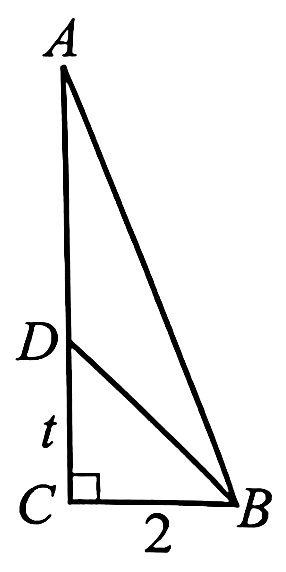
\includegraphics[width=0.14\textwidth]{assets/9-19.jpg}
    \end{vwcol}
\end{enumerate}

\newpage

\section{Induction Formulas of Trigonometric Functions}

In the last section, we discovered that the trigonometric functions of an arbitrary angle are cyclic, and each respective trigonometric value of the angle with the same terminal side is the same. This can be expressed in the following formulas, where $\theta$ is an arbitrary angle, $k \in \mathbb{Z}$, and assuming that the trigonometric functions are defined:

\begin{info}[Trigonometric Values of $\theta + k \cdot 360^\circ$ and $\theta$]
    \begin{align*}
        \sin(\theta + k \cdot 360^\circ) = \sin \theta \qquad \cos(\theta + k \cdot 360^\circ) = \cos \theta \qquad \tan(\theta + k \cdot 360^\circ) = \tan \theta 
    \end{align*}
    \noindent When $k = 1$, we have
    \begin{align*}
        \sin(360^\circ + \theta) = \sin \theta \qquad \cos(360^\circ + \theta) = \cos \theta \qquad \tan(360^\circ + \theta) = \tan \theta
    \end{align*}
\end{info}
With the relationship above, we can convert each trigonometric function to the trigonometric functions of an angle from $0^\circ$ to $360^\circ$ (or $0$ to $2\pi$), then use the reference angle to convert the them to the trigonometric functions of an acute angle to calculate the trigonometric values.

However, apart from using complementary angles, do we have any other ways to convert trigonometric functions of arbitrary angle into trigonometric functions of acute angles for calculation? Actually, we can express an angle whose terminal side lies on the coordinate axes in the form of $k \cdot 90^{\circ}$, so any arbitrary angle can be written as $k \cdot 90^{\circ} \pm \theta$, where $k \in \mathbb{Z}$. If we can find the relationship between the trigonometric values of an arbitrary angle $\theta$ and $k \cdot 90^{\circ} \pm \theta$, we can proceed with the conversion. Next, we are going to explore the relationships between the trigonometric values of $-\theta$, $90^{\circ} \pm \theta$, $180^{\circ} \pm \theta$, $270^{\circ} \pm \theta$, and the trigonometric values of $\theta$.

\begin{explore}[Exploration Activity 2]

\noindent\textbf{Purpose: } To explore trigonometric induction formulas.
\vspace{-1em}
\begin{enumerate}[label=(\alph*)]
    \item Trigonometric Relationship between $-\theta$ and $\theta$
    
    Angles $\theta$ and $-\theta$ represent rotations of the same magnitude but in opposite directions, hence their terminal sides are symmetric about the $x$-axis. Based on the definitions of trigonometric functions for any angle or other methods, find the trigonometric relationship between $-\theta$ and $\theta$.
    \item Trigonometric Relationship between $90^{\circ}+\theta$ and $\theta$
    
    Angle $90^{\circ}+\theta$ differs from angle $\theta$ by $90^{\circ}$. Based on the definition of trigonometric functions or other methods, find the trigonometric relationship between $90^{\circ}+\theta$ and $\theta$.

    \item Trigonometric Relationships between $90^{\circ}-\theta$, $180^{\circ} \pm \theta$, $270^{\circ} \pm \theta$, and $\theta$
    
    Since $90^{\circ}-\theta=90^{\circ}+(-\theta)$, utilize formulas derived from (a) and (b) to find the trigonometric relationship between $90^{\circ}-\theta$ and $\theta$.
    
    Similarly, treat $180^{\circ} \pm \theta$ as $90^{\circ}+\left(90^{\circ} \pm \theta\right)$ and $270^{\circ} \pm \theta$ as $90^{\circ}+\left(180^{\circ} \pm \theta\right)$, we can respectively obtain trigonometric relationships between $180^{\circ} \pm \theta$, $270^{\circ} \pm \theta$, and $\theta$.
\end{enumerate}
\vspace{-1em}
\textbf{Tool: }\url{https://www.geogebra.org/m/w7gx3umv}

\end{explore}

\newpage

From Exploratory Activity 2, we can derive the following formulas. These formulas hold true for any arbitrary θ that makes the trigonometric functions defined.

\begin{center}
    \parbox{0.36\textwidth}{\begin{info}[Trigonometric Values of $-\theta$ and $\theta$]
        \begin{align*}
            \sin(-\theta) &= -\sin \theta\\
            \cos(-\theta) &= \cos \theta\\
            \tan(-\theta) &= -\tan \theta
        \end{align*}
    \end{info}}
\end{center}

\begin{multicols}{2}
    \parbox{0.41\textwidth}{\begin{info}[Trigonometric Values of $90^{\circ} + \theta$ and $\theta$]
        \begin{align*}
            \sin(90^{\circ} + \theta) &= \cos \theta\\
            \cos(90^{\circ} + \theta) &= -\sin \theta\\
            \tan(90^{\circ} + \theta) &= -\cot \theta
        \end{align*}
    \end{info}}
    \parbox{0.41\textwidth}{\begin{info}[Trigonometric Values of $90^{\circ} - \theta$ and $\theta$]
        \begin{align*}
            \sin(90^{\circ} - \theta) &= \cos \theta\\
            \cos(90^{\circ} - \theta) &= \sin \theta\\
            \tan(90^{\circ} - \theta) &= \cot \theta
        \end{align*}
    \end{info}}
\end{multicols}

\begin{multicols}{2}
    \parbox{0.41\textwidth}{\begin{info}[Trigonometric Values of $180^{\circ} + \theta$ and $\theta$]
        \begin{align*}
            \sin(180^{\circ} + \theta) &= -\sin \theta\\
            \cos(180^{\circ} + \theta) &= -\cos \theta\\
            \tan(180^{\circ} + \theta) &= \tan \theta
        \end{align*}
    \end{info}}
    \parbox{0.41\textwidth}{\begin{info}[Trigonometric Values of $180^{\circ} - \theta$ and $\theta$]
        \begin{align*}
            \sin(180^{\circ} - \theta) &= \sin \theta\\
            \cos(180^{\circ} - \theta) &= -\cos \theta\\
            \tan(180^{\circ} - \theta) &= -\tan \theta
        \end{align*}
    \end{info}}
\end{multicols}

\begin{multicols}{2}
    \parbox{0.41\textwidth}{\begin{info}[Trigonometric Values of $270^{\circ} + \theta$ and $\theta$]
        \begin{align*}
            \sin(270^{\circ} + \theta) &= -\cos \theta\\
            \cos(270^{\circ} + \theta) &= \sin \theta\\
            \tan(270^{\circ} + \theta) &= -\cot \theta
        \end{align*}
    \end{info}}
    \parbox{0.41\textwidth}{\begin{info}[Trigonometric Values of $270^{\circ} - \theta$ and $\theta$]
        \begin{align*}
            \sin(270^{\circ} - \theta) &= -\cos \theta\\
            \cos(270^{\circ} - \theta) &= -\sin \theta\\
            \tan(270^{\circ} - \theta) &= \cot \theta
        \end{align*}
    \end{info}}
\end{multicols}

All the formulas in this section are known as the \textbf{induction formulas} of trigonometric functions. This induction formulas can be summarised as follows:

\noindent For the trigonometric values of $k \cdot 90^\circ \pm \theta$ ($k \in \mathbb{Z}$),
\vspace{-1em}
\begin{enumerate}[label=(\roman*)]
    \item When $k$ is even, its value is equal to the value of the function of the same name of theta, adding the sign of the original trigonometric value when treating $\theta$ as an acute angle.
    \item When $k$ odd, its value is equal to the value of the cofunction of theta, adding the sign of the original trigonometric value when treating $\theta$ as an acute angle. ($\sin\alpha$ and $\cos\alpha$, $\tan\alpha$ and $\cot\alpha$, $\sec\alpha$ and $\operatorname{cosec}\alpha$ are cofunctions of each other.)
\end{enumerate}

In the formulas above, changing the sine function to the cosecant function, the cosine function to the secant function, the formulas still hold true. 

\begin{question}
    Simplify the following trigonometric functions into the trigonometric functions of $\theta$:
    \begin{tasks}[label=(\alph*)](2)
            \task $\sec \left(\dfrac{7 \pi}{2}-\theta\right)$
            \task \vspace*{0.5em}$\tan \left(-\theta-180^{\circ}\right)$
        \end{tasks}

    \sol{}
    \begin{enumerate}[label=(\alph*)]
        \item $\begin{aligned}[t] \sec \left(\dfrac{7 \pi}{2}-\theta\right) & =\sec \left[2 \pi+\left(\dfrac{3 \pi}{2}-\theta\right)\right] \\ & =\sec \left(\dfrac{3 \pi}{2}-\theta\right) \\ & =-\operatorname{cosec} \theta\end{aligned}$
        \item $\begin{aligned}[t] \tan \left(-\theta-180^{\circ}\right) & =\tan \left[-\left(\theta+180^{\circ}\right)\right] \\ & =-\tan \left(180^{\circ}+\theta\right) \\ & =-\tan \theta\end{aligned}$
    \end{enumerate}
\end{question}

\practice{9.2a}
Simplify the following trigonometric functions into the trigonometric functions of $\alpha$:

\begin{tasks}[label=(\alph*)](2)
        \task $\sin \left(720^{\circ}-\alpha\right)$
        \task $\cos \left(630^{\circ}+\alpha\right)$
        \task $\tan \left(\dfrac{5 \pi}{2}+\alpha\right)$
        \task $\sec \left(-540^{\circ}+\alpha\right)$
        \task $\operatorname{cosec}(\alpha-7 \pi)$
        \task $\cot \left(-\dfrac{\pi}{2}-\alpha\right)$
    \end{tasks}

    \newpage
    \begin{question}
        Let $A$, $B$, and $C$ be the internal angles of a triangle, prove that $\sin\dfrac{A+B}{2} = \cos\dfrac{C}{2}$.

        \sol{}
        \begin{flalign*}
            & \because A+B+C=180^{\circ} &
        \end{flalign*}
        \vspace{-2.5em}
        \begin{flalign*}
            \therefore \dfrac{A+B}{2}&=\dfrac{180^{\circ}-C}{2} \\
            & =90^{\circ}-\dfrac{C}{2} &
        \end{flalign*}
        \vspace{-2.5em}
        \begin{flalign*}
            \therefore \sin \dfrac{A+B}{2}&=\sin \left(90^{\circ}-\dfrac{C}{2}\right) &\\
            & =\cos \dfrac{C}{2} 
        \end{flalign*}
    \end{question}

    \begin{question}
        Without using a calculator, calculate $\sin 68^{\circ} \sin 22^{\circ}+\cos 112^{\circ} \sin 428^{\circ}$

        \sol{}
        \begin{flalign*}
            \sin 68^{\circ} \sin 22^{\circ}+\cos 112^{\circ} \sin 428^{\circ} & =\sin 68^{\circ} \sin 22^{\circ}+\cos \left(90^{\circ}+22^{\circ}\right) \sin \left(360^{\circ}+68^{\circ}\right) \\ & =\sin 68^{\circ} \sin 22^{\circ}+\left(-\sin 22^{\circ}\right)\left(\sin 68^{\circ}\right) \\ & =0 &
        \end{flalign*}
    \end{question}

    \practice{9.2b}
    \begin{enumerate}
        \item Let $A$, $B$, and $C$ be the internal angles of a triangle, prove the following:
        \begin{tasks}[label=(\alph*)](2)
            \task $\cos (B+C)=-\cos A$
            \task $\cot \dfrac{B+C}{2}=\tan \dfrac{A}{2}$
        \end{tasks}

        \item Without using a calculator, calculate the following:
        \begin{tasks}[label=(\alph*)](2)
            \task $\sin 23^{\circ}-\cos 67^{\circ}$
            \task $\tan 75^{\circ} \tan 15^{\circ}$
        \end{tasks}
    \end{enumerate}

    \newpage

    \exercise{9.2}

    \begin{enumerate}
        \item Simplify the following expressions:
        \begin{tasks}[label=(\alph*)]
            \task $\sin \left(\alpha-180^{\circ}\right)+\tan \left(\alpha-180^{\circ}\right)-\cos \left(90^{\circ}+\alpha\right)$
            \task $\cos (-\alpha) \sec \left(270^{\circ}-\alpha\right)+\dfrac{\sin \left(90^{\circ}-\alpha\right)}{\sin \left(180^{\circ}-\alpha\right)}$
            \task $\dfrac{\cot \left(\dfrac{3 \pi}{2}-\theta\right)+\tan (3 \pi+\theta)}{\sin (2 \pi+\theta) \operatorname{cosec}\left(\dfrac{\pi}{2}-\theta\right)}$
            \task $\sin ^2\left(45^{\circ}+\alpha\right)-\cos ^2\left(45^{\circ}-\alpha\right)$
        \end{tasks}

        \item If $\sin 10^{\circ} = k$, express the following expressions in terms of $k$:
        \begin{tasks}[label=(\alph*)](4)
            \task $\cos 260^{\circ}$
            \task $\sin 280^{\circ}$
            \task $\tan \left(-10^{\circ}\right)$
            \task $\sec 80^{\circ}$
        \end{tasks}
        \item Given $\cos \theta=\dfrac{2}{3}$ and $\theta$ is in the fourth quadrant. Without finding the angle $\theta$, find the value of $\tan \left(180^{\circ}-\theta\right)+\cos \left(90^{\circ}\right)$.
        \item Given $\cot \theta=a$ and $\dfrac{3 \pi}{2}<\theta<2 \pi$, express the following in terms of $a$:
        \begin{tasks}[label=(\alph*)](2)
            \task $\sin (5 \pi+\theta)$
            \task $\operatorname{cosec}\left(-\theta-\dfrac{3 \pi}{2}\right)$
        \end{tasks}
        \item Given that $\dfrac{\sec (\pi-\theta)}{3 \cot \left(\dfrac{\pi}{2}+\theta\right)}=\dfrac{1}{2}$ and $\dfrac{\pi}{2}<\theta<\pi$. Without finding the angle $\theta$, find the value of $\cos \theta$.
    \end{enumerate}

    \section{Graphs of Trigonometric Functions}

    In Exploration Activity 1, we can see that: when the angle $\theta$ changes, the value of its sine, cosine, and tangent functions change accordingly. 

    \subsection*{Graph of Sine Function $y=\sin x$}

    Choosing any angle $x$ in the interval $[0, 2\pi]$, we can find its corresponding sine value $y$. Listed in the table below are the sine values of some special angles:
    
    \SetTblrInner{rowsep=4pt}
    \begin{center}
        \begin{tblr}{|c|c|c|c|c|c|c|c|c|c|c|c|c|c|}
            \hline$x$ & $0$ & $\dfrac{\pi}{6}$ & $\dfrac{\pi}{3}$ & $\dfrac{\pi}{2}$ & $\dfrac{2 \pi}{3}$ & $\dfrac{5 \pi}{6}$ & $\pi$ & $\dfrac{7 \pi}{6}$ & $\dfrac{4 \pi}{3}$ & $\dfrac{3 \pi}{2}$ & $\dfrac{5 \pi}{3}$ & $\dfrac{11 \pi}{6}$ & $2 \pi$ \\
            \hline$y$ & $0$ & $0.5$ & $0.87$ & $1$ & $0.87$ & $0.5$ & $0$ & $-0.5$ & $-0.87$ & $-1$ & $-0.87$ & $-0.5$ & $0$ \\
            \hline
        \end{tblr}
    \end{center}

    Using the corresponding values of each sets of $x$ and $y$ as coordinates, plot these coordinates on the Cartesian plane, and use a smooth curve to connect them, we can obtain the graph of the sine function $y=\sin x$. (As shown in the figure below)
    \vspace{-1em}
    \begin{center}
        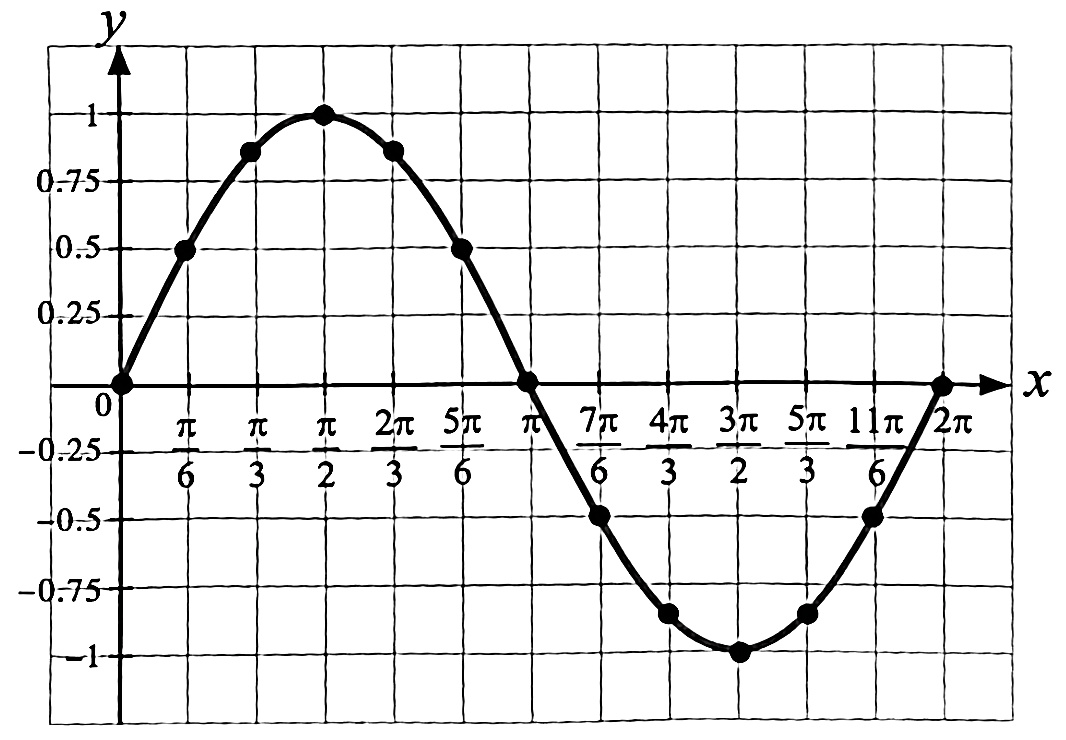
\includegraphics[width=0.4\textwidth]{assets/9-20.jpg}
    \end{center}
    \vspace{-1em}

    From $\sin(2\pi + x) = \sin x$, we know that the sine function $y=\sin x$ will repeat itself every $2\pi$ units. Hence, we can obtain the \text{sine curve} as shown in the figure below. If the value of a function repeats itself after a certain period, we call it a \textbf{periodic function}, and the interval is called the \textbf{period} of the function. The sine function is a periodic function with a minimum positive period of $2\pi$. From now on, when we talk to the period of a function, we usually refer to the minimum positive period of the function.
    \vspace{-1em}
    \begin{center}
        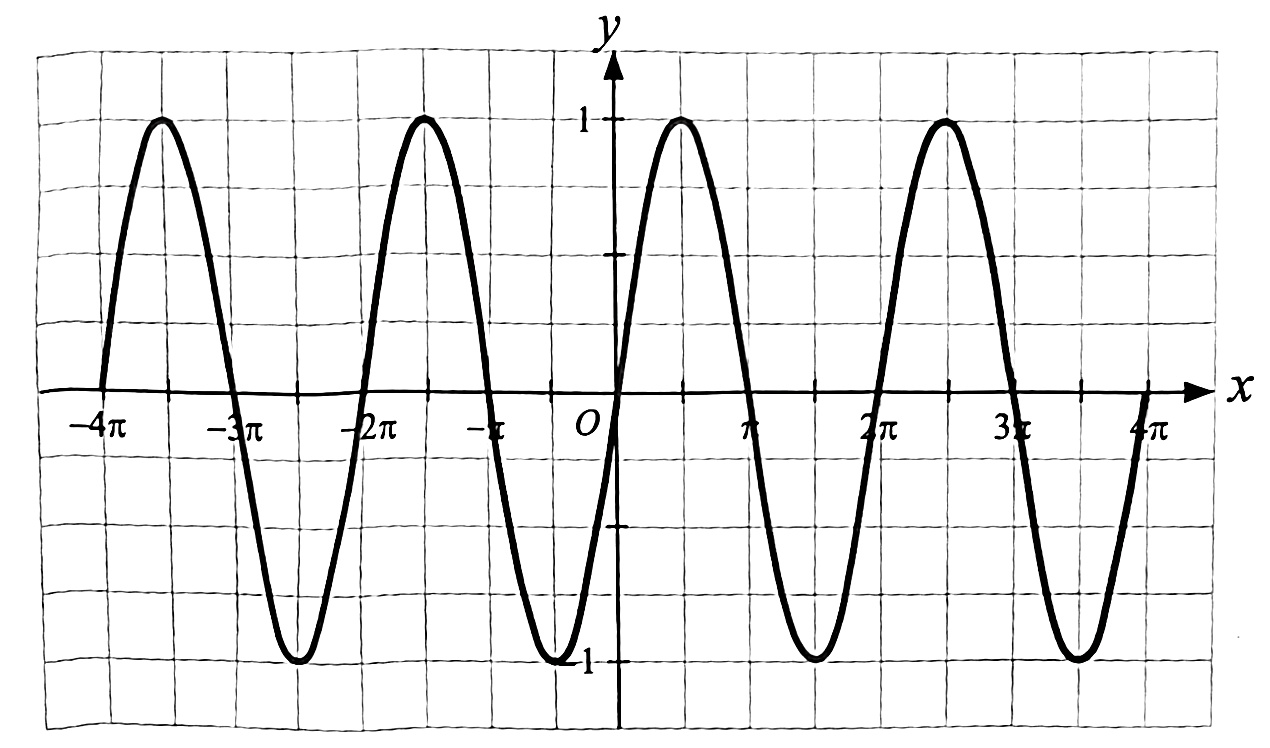
\includegraphics[width=0.5\textwidth]{assets/9-21.jpg}
    \end{center}

    \subsection*{Graph of Cosine Function $y=\cos x$}

    From $\cos(2\pi + x) = \cos x$, we know that the cosine function $y=\cos x$ is also a periodic function with a period of $2\pi$. Base on the periodicity of the function, we can list down the coordinates and plot them on the Cartesian plane to obtain the graph of the cosine function $y=\cos x$. (As shown in the figure below)
    
    \begin{center}
        \begin{tblr}{|c|c|c|c|c|c|c|c|c|c|c|c|c|c|}
            \hline$x$ & $0$ & $\dfrac{\pi}{6}$ & $\dfrac{\pi}{3}$ & $\dfrac{\pi}{2}$ & $\dfrac{2 \pi}{3}$ & $\dfrac{5 \pi}{6}$ & $\pi$ & $\dfrac{7 \pi}{6}$ & $\dfrac{4 \pi}{3}$ & $\dfrac{3 \pi}{2}$ & $\dfrac{5 \pi}{3}$ & $\dfrac{11 \pi}{6}$ & $2 \pi$ \\
            \hline $y$ & $1$ & $0.87$ & $0.5$ & $0$ & $-0.5$ & $-0.87$ & $-1$ & $-0.87$ & $-0.5$ & $0$ & $0.5$ & $-0.87$ & $1$ \\
            \hline
        \end{tblr}
    \end{center}

        \begin{center}
            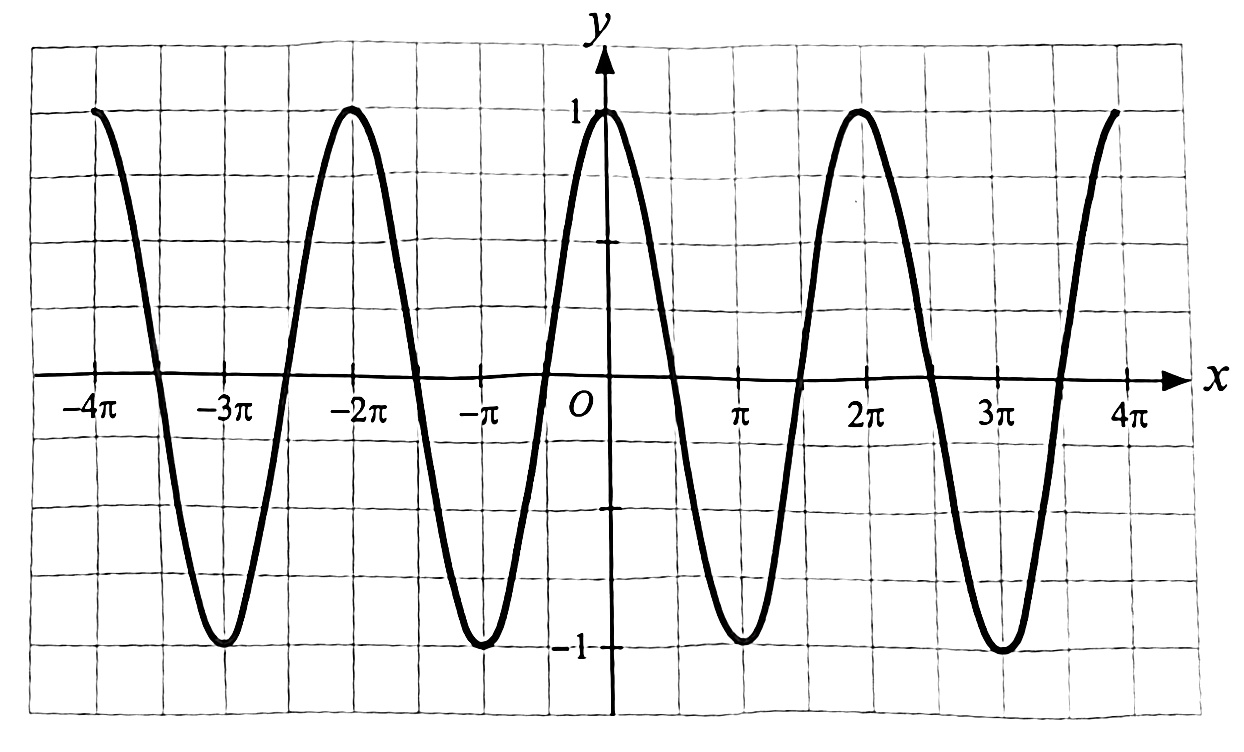
\includegraphics[width=0.5\textwidth]{assets/9-22.jpg}
        \end{center}

        Comparing the graph of the sine and cosine functions, we can see that there are a lot of similarities between them. We only have to translate the sine curve $\dfrac{\pi}{2}$ units to the left to obtain the cosine curve.

        \subsection*{Graph of Tangent Function $y=\tan x$}

        From $\tan (\pi+x)=\tan x$, we know that $y=\tan x$ is a function with a period of $\pi$. The figure below shows the tangent curve. The dashed lines in the figure represent asymptotes. Since $\tan x$ is undefined at $-\dfrac{3 \pi}{2},-\dfrac{\pi}{2}$, $\dfrac{\pi}{2}$, and $\dfrac{3 \pi}{2}$, the tangent curve discontinuities at these angles. As $x$ approaches these angles, the graph of $y=\tan x$ extends indefinitely at both ends.
        \begin{center}
            \begin{tblr}{|c|c|c|c|c|c|c|c|c|c|}
                    \hline$x$ & $-\dfrac{\pi}{2}$ & $-\dfrac{\pi}{3}$ & $-\dfrac{\pi}{4}$ & $-\dfrac{\pi}{6}$ & $0$ & $\dfrac{\pi}{6}$ & $\dfrac{\pi}{4}$ & $\dfrac{\pi}{3}$ & $\dfrac{\pi}{2}$ \\
                   \hline y & undefined & $-1.73$ & $-1$ & $-0.58$ & $0$ & $0.58$ & $1$ & $1.73$ & undefined\\
                    \hline
            \end{tblr}
        \end{center}
        \begin{center}
            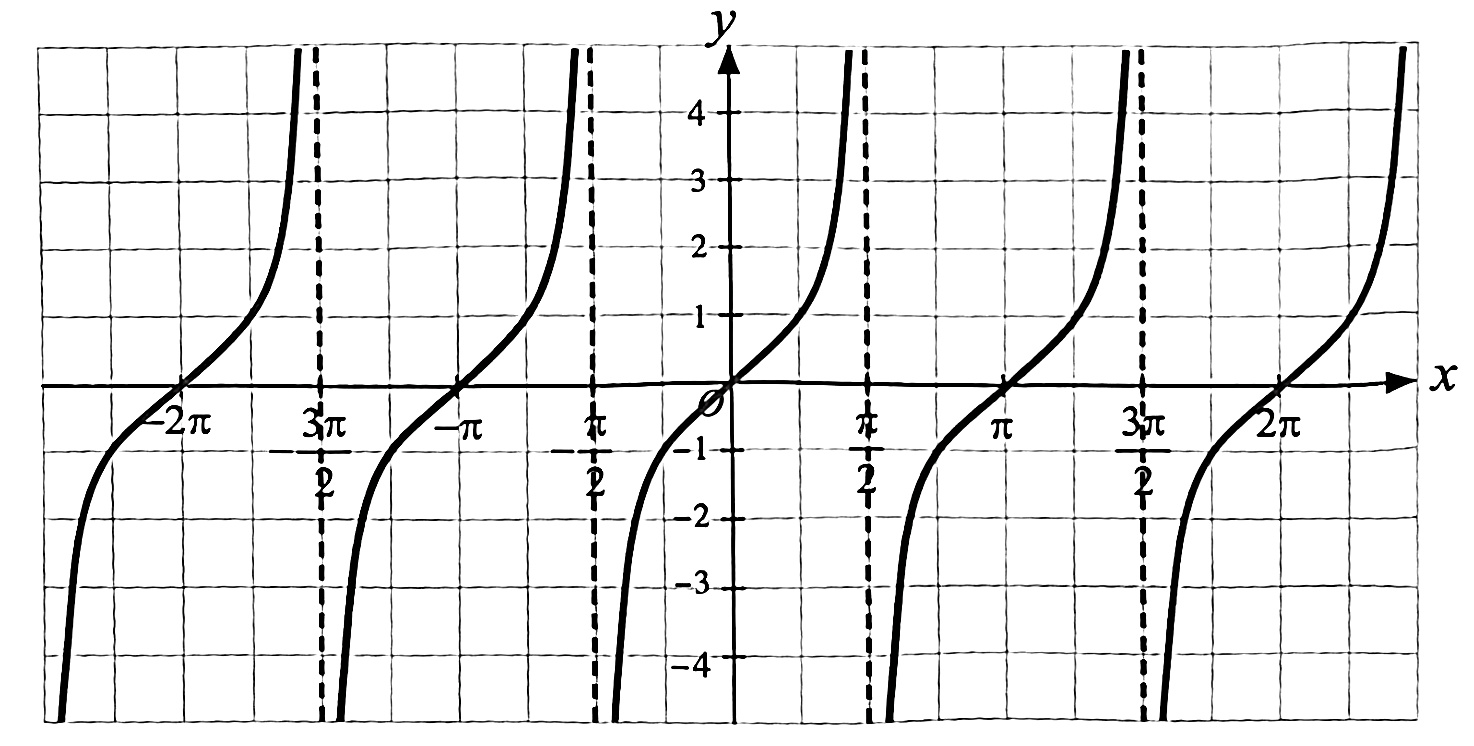
\includegraphics[width=0.5\textwidth]{assets/9-23.jpg}
        \end{center}

        \practice{9.3a}
        
        Sketch the simplified graphs of the following trigonometric functions:
        \begin{tasks}[label=(\alph*)](2)
            \task $y=\cos x$ ($-\pi \leq x \leq \pi$)
            \task $y=\tan x$ ($-pi \leq x \leq \pi$)
        \end{tasks}

        \newpage
        \subsection*{Properties of Trigonometric Functions}

        From the definitions and the graphs of the trigonometric functions, we can observe a few properties of the sine, cosine, and tangent functions, as listed below:
        \begin{center}
            \begin{tblr}{|c|c|c|}
                \hline Function & $y=\sin x \quad y=\cos x$ & $y=\tan x$ \\
                \hline Domain & $\mathbb{R}$ & $\left\{x \left\lvert\, x \neq k \pi+\dfrac{\pi}{2}\right., k \in \mathbb{Z}\right\}$ \\
                \hline Range & {$[-1,1]$} & $\mathbb{R}$ \\
                \hline Minimum Positive Period & $2 \pi$ & $\pi$ \\
                \hline
            \end{tblr}
        \end{center}

        For any real number $x$, $-1 \leq \sin x \leq 1$, hence the maximum value of $\sin x$ is 1, and the minimum value is -1. From the graph of the sine function, we can see that at $x = 2k\pi + \dfrac{\pi}{2}$, $k \in \mathbb{Z}$, $\sin $ has a maximum value of 1; at $x = 2k\pi - \dfrac{\pi}{2}$, $k \in \mathbb{Z}$, $\sin $ has a minimum value of -1. Similarly, $\cos x$ has a maximum value of 1 at $x = 2k\pi$, $k \in \mathbb{Z}$, and a minimum value of -1 at $x = (2k + 1)\pi$, $k \in \mathbb{Z}$.
        
        The graphs of the sine and cosine functions are wave-shaped curves. We can observe that the amplitudes of the wave-shaped curves of $y=\sin x$ and $y=\cos x$ are both 1, meaning the maximum distance of the curves from the equilibrium position (the $x$-axis) is 1.

        Unlike the sine and cosine functions, $\tan x$ can take any real value, so the tangent function does not have a maximum or minimum value.

        \practice{9.3b}
        Can the following expressions hold true? Why?
        \begin{tasks}[label=(\alph*)](2)
            \task $\cos ^2 x=1.5$
            \task $3 \sin x=5$
            \task $\sin x-\cos x=2$
            \task $\tan x+\cot x=2$
        \end{tasks}

        \newpage
        \subsection*{Transformations of Trigonometric Functions}

        A lot of periodic phenomena are often represented using sine and cosine curves. For example, alternating current, which varies sinusoidally with time $t$, can be expressed as $I=I_m \sin \omega t$, where $I_m$ is the maximum current intensity, and $\omega$ is the angular velocity of the generator's coil rotation. Now, we will further study the graphs of more complex trigonometric functions using the function transformations learned in Chapter 5.

        Now, we will illustrate how to draw the graphs of (i) $y=a \sin x$, (ii) $y=\sin b x(b>0)$, (iii) $y=\sin (x+c)$, and (iv) $y=\sin x+d$ using $y=\sin x$ as the base function.

        \vspace{-1em}
        \subsubsection*{(i) Graph of $\mathbf{y=a \text{ sin } x}$}
        
        Let's first study the graph of $y=3 \sin x$.

        As shown in the table below, for any value of $x$, the value of $3 \sin x$ is three times the value of $\sin x$. The function $y=3 \sin x$ is another wave-shaped curve, with an amplitude of 3 and a minimum positive period of $2 \pi$. The coefficient 3 simply increases the height of the sine curve to three times its original height without affecting its period. (See the figure below).

        \begin{tblr}{|c|c|c|c|c|c|c|c|c|c|c|c|c|c|c|c|}
            \hline$x$ & $\cdots$ &  $0$& $\dfrac{\pi}{6}$ & $\dfrac{\pi}{3}$ & $\dfrac{\pi}{2}$ & $\dfrac{2 \pi}{3}$ & $\dfrac{5 \pi}{6}$ & $\pi$ & $\dfrac{7 \pi}{6}$ & $\dfrac{4 \pi}{3}$ & $\dfrac{3 \pi}{2}$ & $\dfrac{5 \pi}{3}$ & $\dfrac{11 \pi}{6}$ & $2 \pi$ & $\cdots$ \\
            \hline $\sin x$ & $\cdots$ & $0$ & $0.5$ & $0.87$ & $1$ & $0.87$ & $0.5$ & $0$ & $-0.5$ & $-0.87$ & $-1$ & $-0.87$ & $-0.5$ & $0$ & $\cdots$ \\
            \hline $3 \sin x$ & $\cdots$ & $0$ & $1.5$ & $2.6$ & $3$ & $2.6$ & $1.5$ & $0$ & $-1.5$ & $-2.6$ & $-3$ & $-2.6$ & $-1.5$ & $0$ & $\cdots$ \\
            \hline
        \end{tblr}
        \begin{center}
            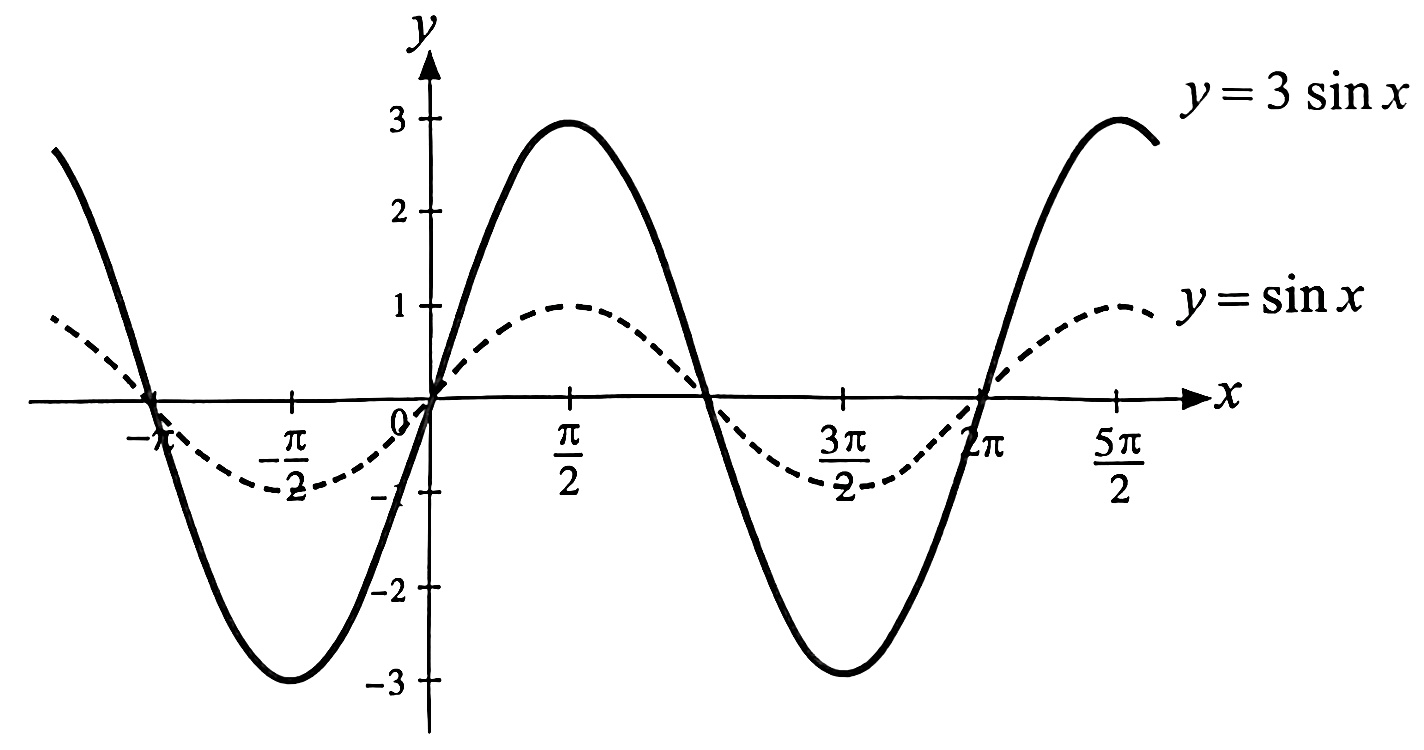
\includegraphics[width=0.5\textwidth]{assets/9-24.jpg}
        \end{center}

        \vspace{-1em}
        \subsubsection*{(ii) Graph of $\mathbf{y=\text{ sin } b x\ (b>0)}$}

        Next, let's study the graph of $y=\sin 2x$.

        As shown in the table bwlow, for any value of $x$, the value of $\sin 2x$ is the value of $\sin x$ when $x$ is multiplied by 2.
        \begin{center}
            \begin{tblr}{|c|c|c|c|c|c|c|c|c|c|c}
                \hline$x$ & $\cdots$ & $0$ & $\dfrac{\pi}{16}$ & $\dfrac{\pi}{8}$ & $\dfrac{\pi}{4}$ & $\dfrac{\pi}{2}$ & $\pi$ & $2 \pi$ & $\ldots$ \\
                \hline  $\sin x$ & $\cdots$ & $0$ & $\sin \dfrac{\pi}{16}$ & $\sin \dfrac{\pi}{8}$ & $\sin \dfrac{\pi}{4}$ & $\sin \dfrac{\pi}{2}$ & $\sin \pi$ & $\sin 2 \pi$ & $\ldots$ \\
                \hline $\sin 2 x$ & $\cdots$ & $0$ & $\sin \dfrac{\pi}{8}$ & $\sin \dfrac{\pi}{4}$ & $\sin \dfrac{\pi}{2}$ & $\sin \pi$ & $\sin 2 \pi$ & $\sin 4 \pi$ & $\ldots$ \\
                \hline
            \end{tblr}
        \end{center}

        This indicates that $y=\sin 2 x$ has the same values as $y=\sin x$ but with interval half as short (changing twice as fast). The function $y=\sin 2 x$ is another sine wave curve, with an amplitude of 1, but its minimum positive period is $\dfrac{2 \pi}{2}=\pi$. The coefficient of $x$ 2 compresses the curve horizontally (along the $x$-axis) on either side of the origin to $\dfrac{1}{2}$ of its original width. The period of the function $\sin 2 x$ is half that of $\sin x$. (See the figure below).
        \begin{center}
            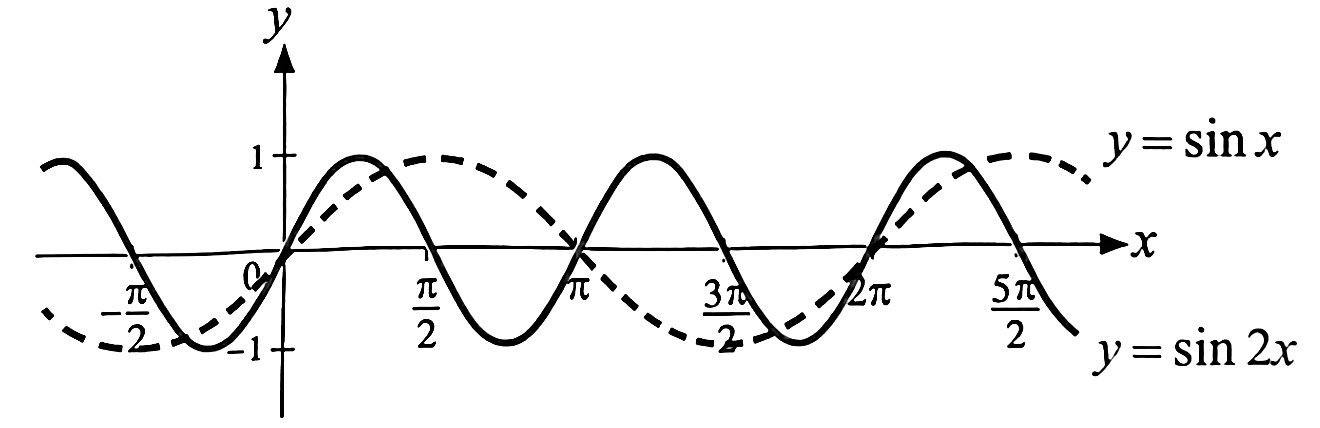
\includegraphics[width=0.5\textwidth]{assets/9-25.jpg}
        \end{center}

        Generally, since $\sin b\left(x+\dfrac{2 \pi}{b}\right)=\sin b x$, the period of $\sin b x$ is $\dfrac{2 \pi}{b}$. When $b>1$, its graph is formed by compressing the graph of $y=\sin x$ towards the origin along the $x$-axis, with its period being $\dfrac{1}{b}$ of the original period. As $b$ increases, the period decreases.

        \begin{question}
            Sketch the graph of $y=3\sin 2x$.

            \sol{}

            \noindent The graph of $y=3 \sin 2 x$ is a combination of the graphs we previously studied, $y=3 \sin x$ and $y=\sin 2 x$. It can be observed that this is a sine wave curve with an amplitude of 3 and a period of $\dfrac{2 \pi}{2}=\pi$, as shown in the following graph.
            \vspace{-1.5em}
            \begin{center}
                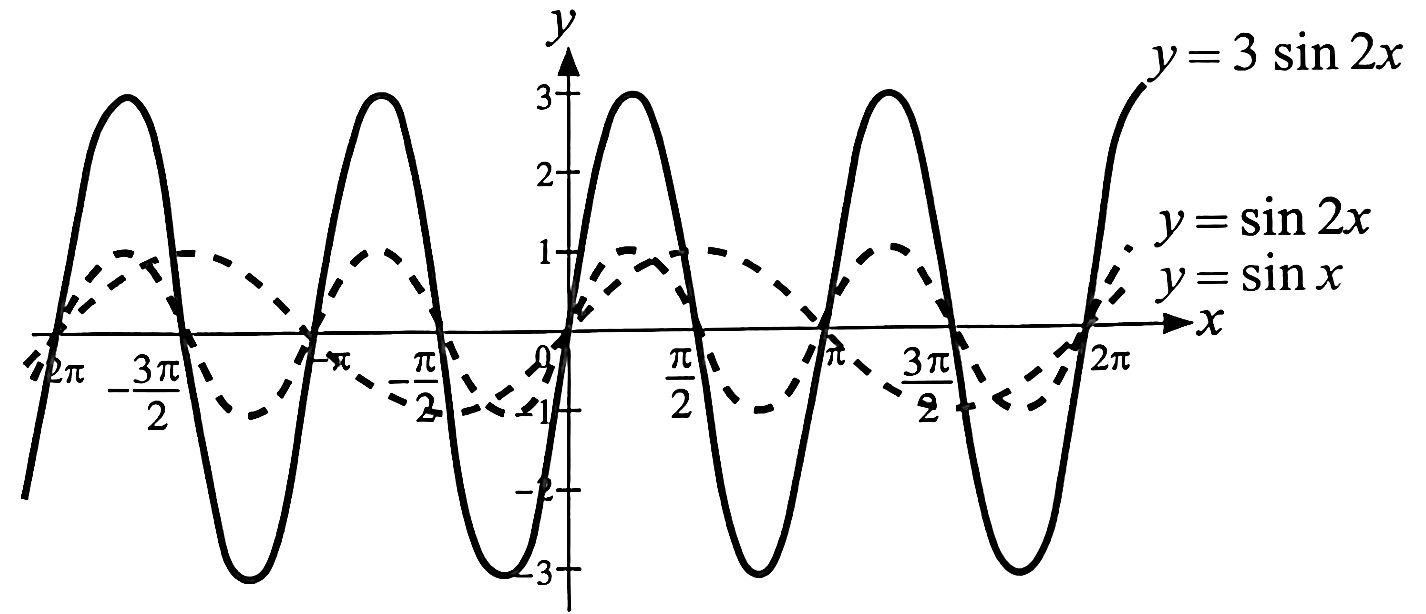
\includegraphics[width=0.5\textwidth]{assets/9-26.jpg}
            \end{center}
        \end{question}

        \vspace{-1.5em}
        \subsubsection*{(iii) Graph of $\mathbf{y=\text{ sin }(x+c)}$}

        Now, let's study the graph of $y=\sin (x+\dfrac{\pi}{6})$.

        Let's define some values of $x$ and compare the values of $y = \sin\left(x+\dfrac{\pi}{6}\right)$ with the values of $y = \sin x$, as shown in the table below.
        \begin{center}
            \begin{tblr}{|c|c|c|c|c|c|c|c|c|c|c|c|c|c|}
                \hline$x$ & $\cdots$ & $0$ & $\dfrac{\pi}{12}$ & $\dfrac{\pi}{6}$ & $\dfrac{\pi}{4}$ & $\dfrac{\pi}{3}$ & $\dfrac{5 \pi}{12}$ & $\dfrac{\pi}{2}$ & $\dfrac{7 \pi}{12}$ & $\dfrac{2 \pi}{3}$ & $\dfrac{3 \pi}{4}$ & $\dfrac{5 \pi}{6}$ & $\ldots$ \\
                \hline $\sin x$ & $\cdots$ & $0$ & $0.26$ & $\dfrac{1}{2}$ & $\dfrac{\sqrt{2}}{2}$ & $\dfrac{\sqrt{3}}{2}$ & $0.97$ & $1$ & $0.97$ & $\dfrac{\sqrt{3}}{2}$ & $\dfrac{\sqrt{2}}{2}$ & $\dfrac{1}{2}$ & $\ldots$ \\
                \hline $\sin \left(x+\dfrac{\pi}{6}\right)$ & $\cdots$ & $\dfrac{1}{2}$ & $\dfrac{\sqrt{2}}{2}$ & $\dfrac{\sqrt{3}}{2}$ & $0.97$ & $1$ & $0.97$ & $\dfrac{\sqrt{3}}{2}$ & $\dfrac{\sqrt{2}}{2}$ & $\dfrac{1}{2}$ & $0.26$ & $0$ & $\ldots$ \\
                \hline
                \end{tblr}
        \end{center}

        It can be seen that in $y=\sin \left(x+\dfrac{\pi}{6}\right)$, the values of $y$ are the same as in $y=\sin x$, but the starting point is different, being at $\dfrac{\pi}{6}$ units before the corresponding values in $y=\sin x$. Therefore, to obtain the graph of $y=\sin \left(x+\dfrac{\pi}{6}\right)$, we just need to shift the graph of $y=\sin x$ to the left by $\dfrac{\pi}{6}$. (See the figure below).
        \begin{center}
            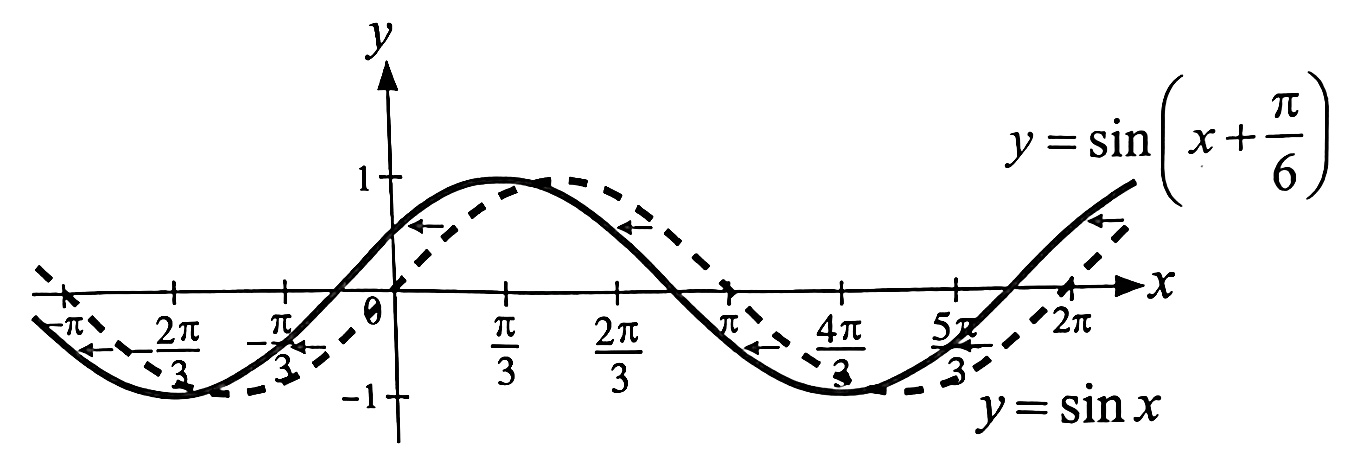
\includegraphics[width=0.5\textwidth]{assets/9-27.jpg}
        \end{center}

        Generally, to obtain the graph of $y=\sin (x+c)$, we can shift the graph of $y=\sin x$ by a distance of $|c|$. If $c$ is positive, the graph is shifted to the left; if $c$ is negative, it is shifted to the right.
        
        \begin{question}
            Sketch the graph of $y=\sin \left(2x + \dfrac{\pi}{3}\right)$.

            \sol{}
            
            \noindent Since $y = \sin\left(2x + \dfrac{\pi}{3}\right) = \sin 2\left(x + \dfrac{\pi}{6}\right)$, 
            \begin{enumerate}[label=(\arabic*), leftmargin=*, topsep=0pt]
                \item By compressing the graph of $y=\sin x$ along the $x$-axis such that the period becomes half of the original, we obtain the graph of $y=\sin 2 x$.
                \item By shifting the graph of $y=\sin 2 x$ to the left by $\dfrac{\pi}{6}$, we obtain the graph of $y=\sin 2\left(x+\dfrac{\pi}{6}\right)$, i.e. the graph of $y=\sin \left(2 x+\dfrac{\pi}{3}\right)$.
            \end{enumerate}
            \begin{center}
                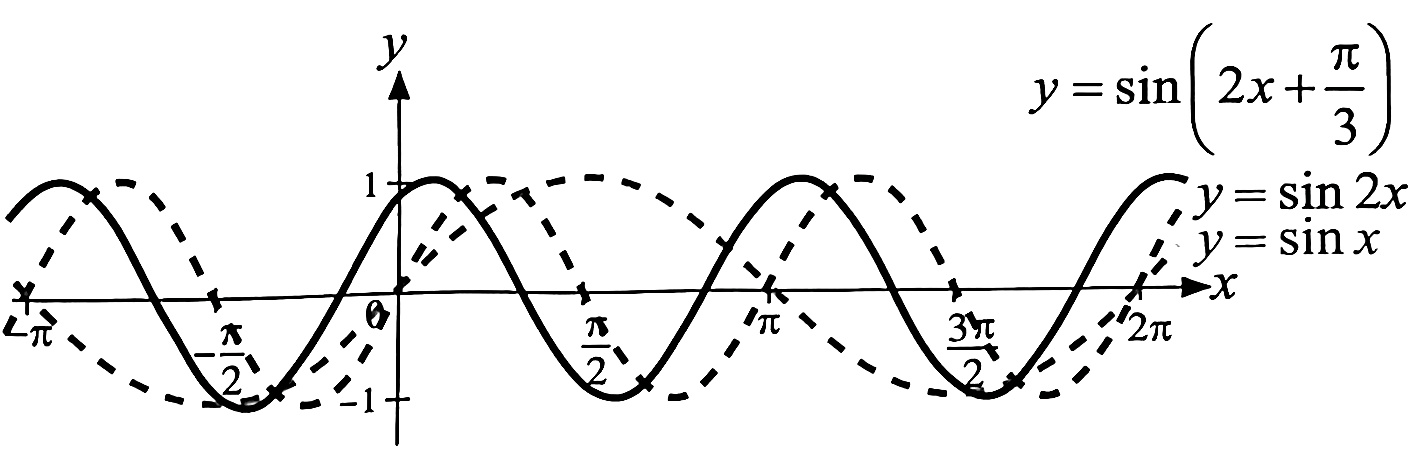
\includegraphics[width=0.5\textwidth]{assets/9-28.jpg}
            \end{center}
        \end{question}
        \begin{think}
            
            \noindent How to sketch the graph of $y=\sin \left(2x+\dfrac{\pi}{3}\right)$ from the graph of $y=\sin \left(x+\dfrac{\pi}{3}\right)$?
        \end{think}

        \newpage
        \subsubsection*{(iv) Graph of $\mathbf{y=\text{ sin } x+d}$}

        Let's study the graph of $y=\sin x+2$.

        As shown in the table below, for any value of $x$, the value of $\sin x+2$ is equal to the value of $\sin x$ plus 2. We can obtain the graph of $y=\sin x+2$ by shifting the graph of $y=\sin x$ upward by 2 units. (See the figure below)
        \begin{center}
            \begin{tblr}{|c|c|c|c|c|c|c|c|c|c|c|c|c|c|c|c|}
                \hline$x$ & $\cdots$ & $0$ & $\dfrac{\pi}{6}$ & $\dfrac{\pi}{3}$ & $\dfrac{\pi}{2}$ & $\dfrac{2 \pi}{3}$ & $\dfrac{5 \pi}{6}$ & $\pi$ & $\dfrac{7 \pi}{6}$ & $\dfrac{4 \pi}{3}$ & $\dfrac{3 \pi}{2}$ & $\dfrac{5 \pi}{3}$ & $\dfrac{11 \pi}{6}$ & $2 \pi$ & $\cdots$ \\
                \hline $\sin x$ & $\cdots$ & $0$ & $0.5$ & $0.87$ & $1$ & $0.87$ & $0.5$ & $0$ & $-0.5$ & $-0.87$ & $-1$ & $-0.87$ & $-0.5$ & $0$ & $\cdots$ \\
                \hline $\sin x+2$ & $\cdots$ & $2$ & $2.5$ & $2.87$ & $3$ & $2.87$ & $2.5$ & $2$ & $1.5$ & $1.13$ & $1$ & $1.13$ & $1.5$ & $2$ & $\cdots$ \\
                \hline
                \end{tblr}
        \end{center}
        \begin{center}
            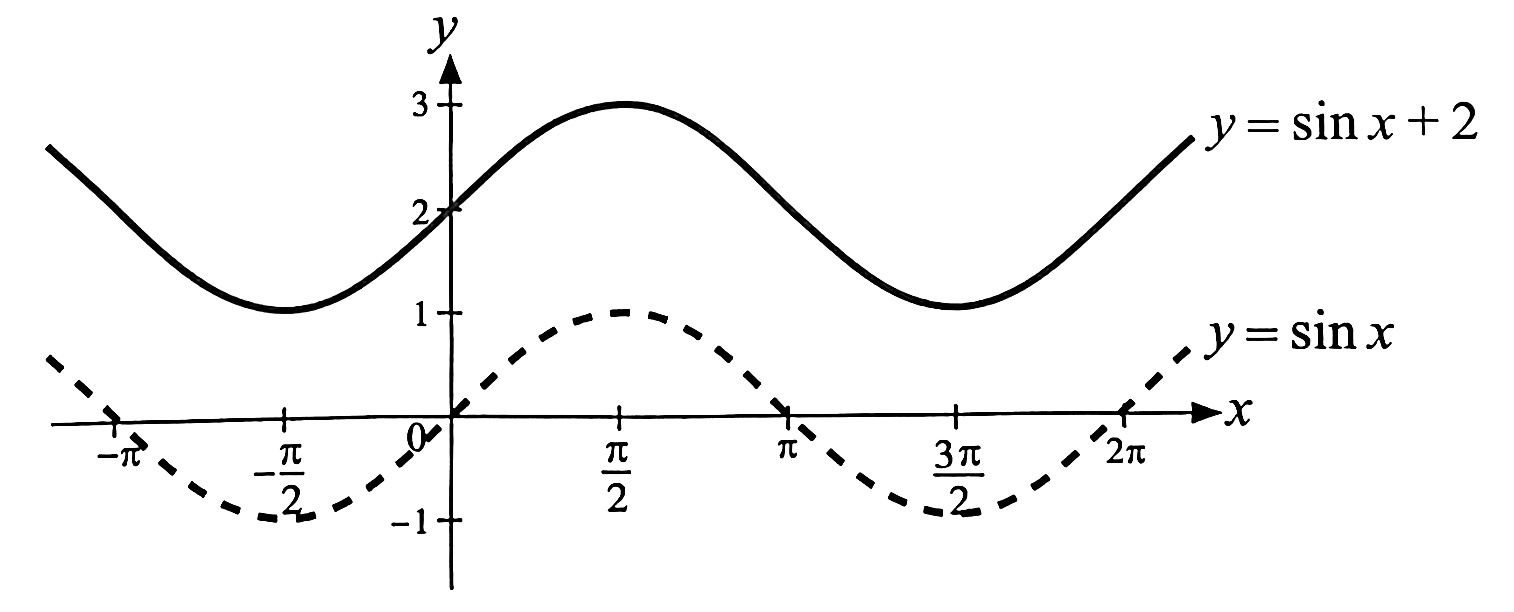
\includegraphics[width=0.5\textwidth]{assets/9-29.jpg}
        \end{center}

        After the four transformations mentioned above, we can plot the graph of $y=a \sin (b x+c)+d$ from the function $y=\sin x$, where $a, c, d$ are real numbers and $b$ is a positive real number. By applying these transformations, we can also draw graphs of other complex trigonometric functions such as cosine and tangent functions. The table below summarizes the effects of parameters $a, b, c$, and $d$ on the graph transformation of the trigonometric function $y=f(x)$:

        \begin{center}
            \begin{tabular}{|c|c|c|c|}
                \hline Functions & Parameters & Changes of Graph & Transformations \\
                \hline \multirow{2}{*}{\parbox{0.088\textwidth}{\vspace{1.8em}$y=a f(x)$}} & $0<a<1$ & \parbox{0.4\textwidth}{\vspace{0.5em}The ordinate of each point is compressed by a factor of $a$.\vspace{0.5em}} & \multirow{2}{*}{\parbox{0.16\textwidth}{\vspace{1.8em}\centering Stretch Vertically}} \\
                \cline{2-3} & $a>1$ & \parbox{0.4\textwidth}{\vspace{0.5em}The ordinate of each point is stretched by a factor of $a$.\vspace{0.5em}} & \\
                \hline \multirow{2}{*}{\begin{tabular}{c}
                    \parbox{0.1\textwidth}{\vspace{1.8em}\centering $y=f(b x)$ \\
                $b>0$}
                \end{tabular}} & $0<b<1$ & \parbox{0.4\textwidth}{\vspace{0.5em}The abscissa of each point is stretched by a factor of $\dfrac{1}{b}$.\vspace{0.5em}} & \multirow{2}{*}{\parbox{0.18\textwidth}{\vspace{1.8em}\centering Stretch Horizontally}} \\
                \cline{2-3} & $b>1$ & \parbox{0.4\textwidth}{\vspace{0.5em}The abscissa of each point is stretched by a factor of $\dfrac{1}{b}$.\vspace{0.5em}} & \\
                \hline \multirow{2}{*}{\parbox{0.1\textwidth}{\vspace{0.7em}\centering $y=f(x+c)$}} & $c<0$ & \parbox{0.4\textwidth}{\vspace{0.5em}Each point is shifted to the right by $|c|$ units.\vspace{0.5em}} & \multirow{2}{*}{\parbox{0.16\textwidth}{\vspace{0.7em}\centering Shift Horizontally}} \\
                \cline{2-3} & $c>0$ & \parbox{0.4\textwidth}{\vspace{0.5em}Each point is shifted to the left by $|c|$ units.\vspace{0.5em}} & \\
                \hline \multirow{2}{*}{\parbox{0.1\textwidth}{\vspace{0.7em}\centering $y=f(x)+d$}} & $d<0$ & \parbox{0.4\textwidth}{\vspace{0.5em}Each point is shifted to the bottom by $|c|$ units.\vspace{0.5em}} & \multirow{2}{*}{
                    \parbox{0.16\textwidth}{\vspace{0.7em}\centering Shift Vertically}} \\
                \cline{2-3} & $d>0$ & \parbox{0.4\textwidth}{\vspace{0.5em}Each point is shifted to the top by $|c|$ units.\vspace{0.5em}} & \\
                \hline
                \end{tabular}
        \end{center}

        \begin{question}
            Sketch the graph of $y=\cos \left(x-\dfrac{\pi}{4}\right)$, and state its relationship with the graph of $y=\cos x$.
            
            \sol{}
            \begin{center}
                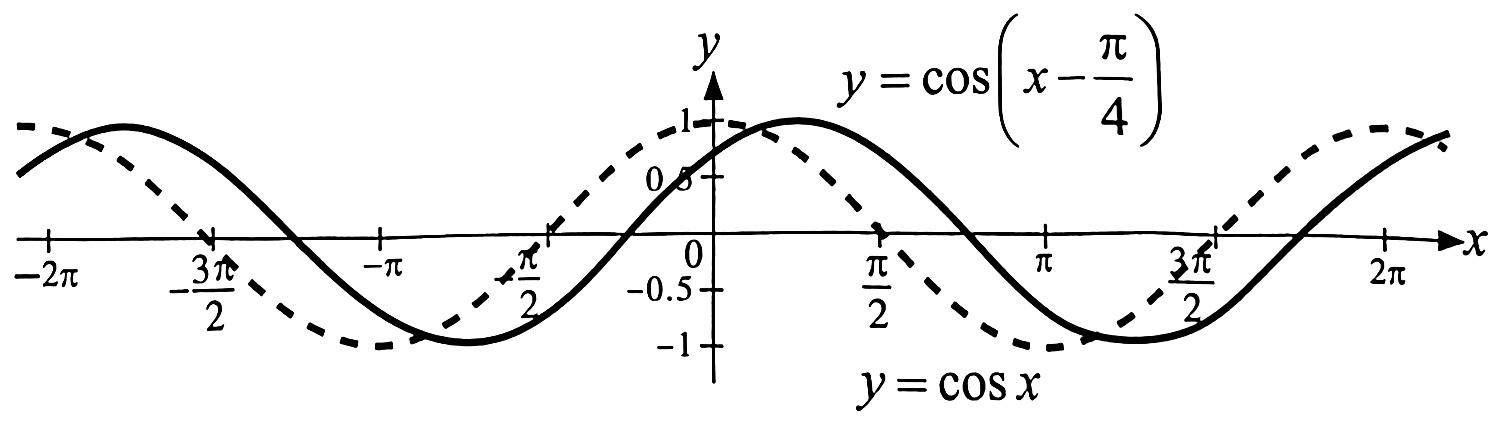
\includegraphics[width=0.6\textwidth]{assets/9-30.jpg}
            \end{center}
            \vspace{-1.5em}
            The graph of $y=\cos \left(x-\dfrac{\pi}{4}\right)$ is obtained by shifting the graph of $y=\cos x$ to the right by $\dfrac{\pi}{4}$ units along the $x$-axis.
        \end{question}
        \vspace{-1em}
        \begin{question}
            The graph below shows a segment of the function $y = a \cos(bx + c) + d$. Determine the function.
            \begin{center}
                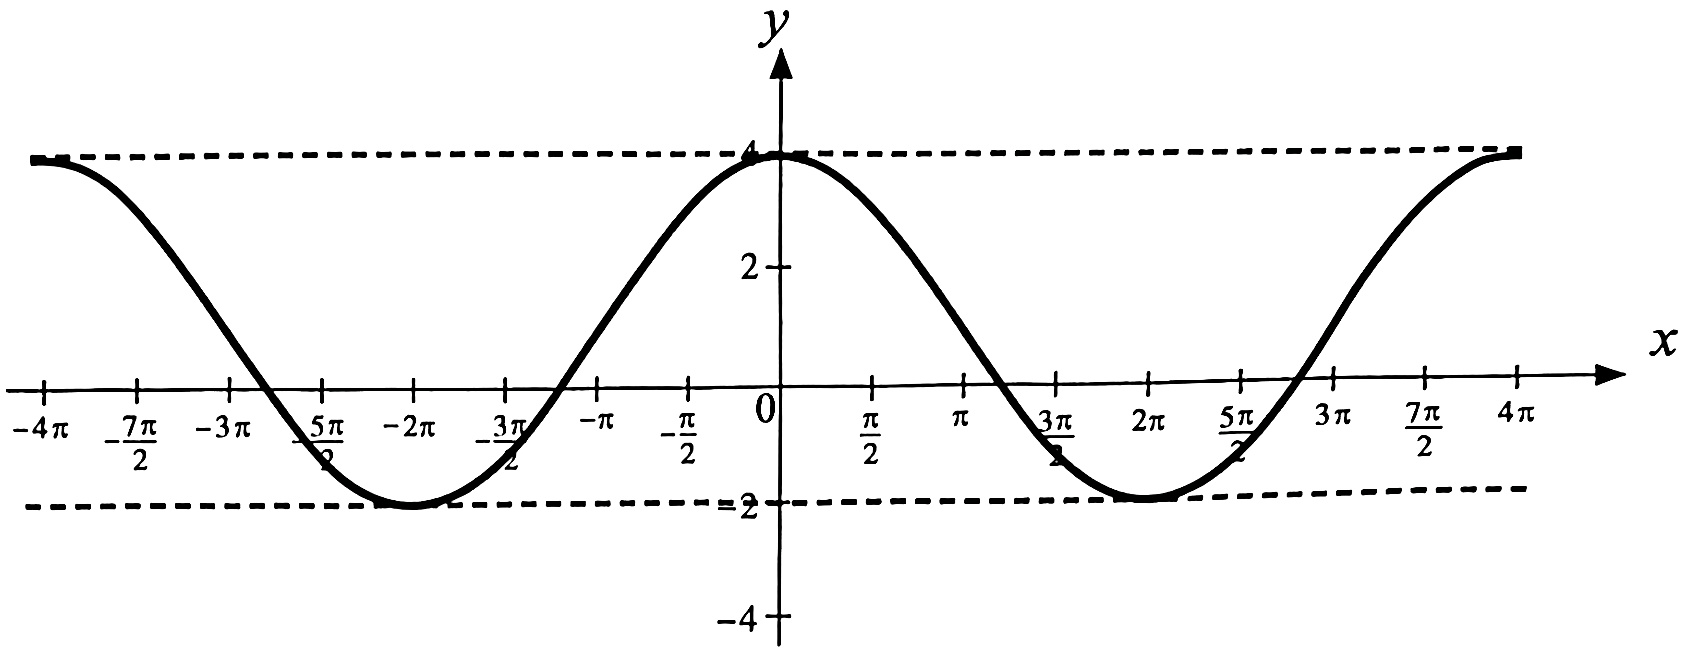
\includegraphics[width=0.6\textwidth]{assets/9-31.jpg}
            \end{center}
            \vspace{-2em}
            \sol{}

            \noindent The amplitude $=\dfrac{4-(-2)}{2}=3$. Hence, $a=3$. 
            
            \vspace{-1em}
            \noindent The minimum positive period of the graph is $4\pi$. From $\dfrac{2\pi}{b}=4\pi$, we get $b=\dfrac{1}{2}$. 
            
            \vspace{-1em}
            \noindent Comparing with $y=3\cos\dfrac{x}{2}$, there is no left or right shift, hence $c=0$. 
            
            \vspace{-1em}
            \noindent From the point $(0,4)$, by letting $4=3\cos 0+d$, we get $d=1$. 
            
            \vspace{-1em}
            \noindent Thus, the function representing the graph is $y=3\cos\dfrac{x}{2}+1$.
            
        \end{question}
        \vspace{-3em}
        \practice{9.3c}
        \begin{enumerate}
            \item Find the amplitude and period of the following functions, and explain how to transform the graph of $y=\sin x$to obtain the graphs of the following functions. Hence, sketch simple graphs of the following functions.
            \begin{tasks}[label=(\alph*)](2)
                \task $y=6 \sin x$
                \task $y=\sin \left(x-\dfrac{\pi}{3}\right)$
            \end{tasks}
            \vspace{-1em}
            \begin{multicols}{2}
                \item The graph on the right is the plot of the function $y=a \sin b x, b>0$. Find the values of $a$ and $b$.

                \begin{center}
                    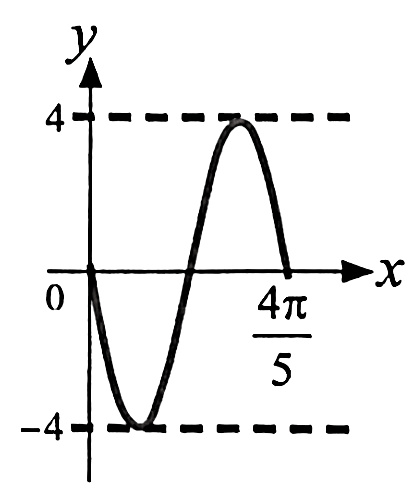
\includegraphics[width=0.15\textwidth]{assets/9-32.jpg}
                \end{center}
            \end{multicols}
            \vspace{-2em}
        \end{enumerate}

        \newpage
        \exercise{9.3}
        \begin{enumerate}
            \item Sketch the following trigonometric functions:
            \begin{tasks}[label=(\alph*)](2)
                \task \( y=|\sin x| \quad(-\pi \leq x \leq \pi) \)
                \task \( y=-\tan x \quad(0 \leq x \leq 2 \pi) \)
            \end{tasks}
            \item Find the maximum and minimum values of the following functions:
            \begin{tasks}[label=(\alph*)](2)
                \task \( f(x)=2 \cos x-3 \)
                \task \( f(x)=\dfrac{6}{3-\sin x} \)
            \end{tasks}
            \item  Plot the following functions in order in the same Cartesian coordinate system on the interval \( -2 \pi \leq x \leq 2 \pi \). Hence, find their ranges:
            \begin{tasks}[label=(\alph*)](2)
                \task \( y=\sin 3 x \)
                \task \( y=\sin \left(3 x+\dfrac{\pi}{2}\right) \)
                \task \( y=4 \sin \left(3 x+\dfrac{\pi}{2}\right) \)
                \task \( y=3+4 \sin \left(3 x+\dfrac{\pi}{2}\right) \)
            \end{tasks}
            \item The figure below shows the graph of the function \( y=a \cos b x+c, b>0 \). Find this function.
            \begin{center}
                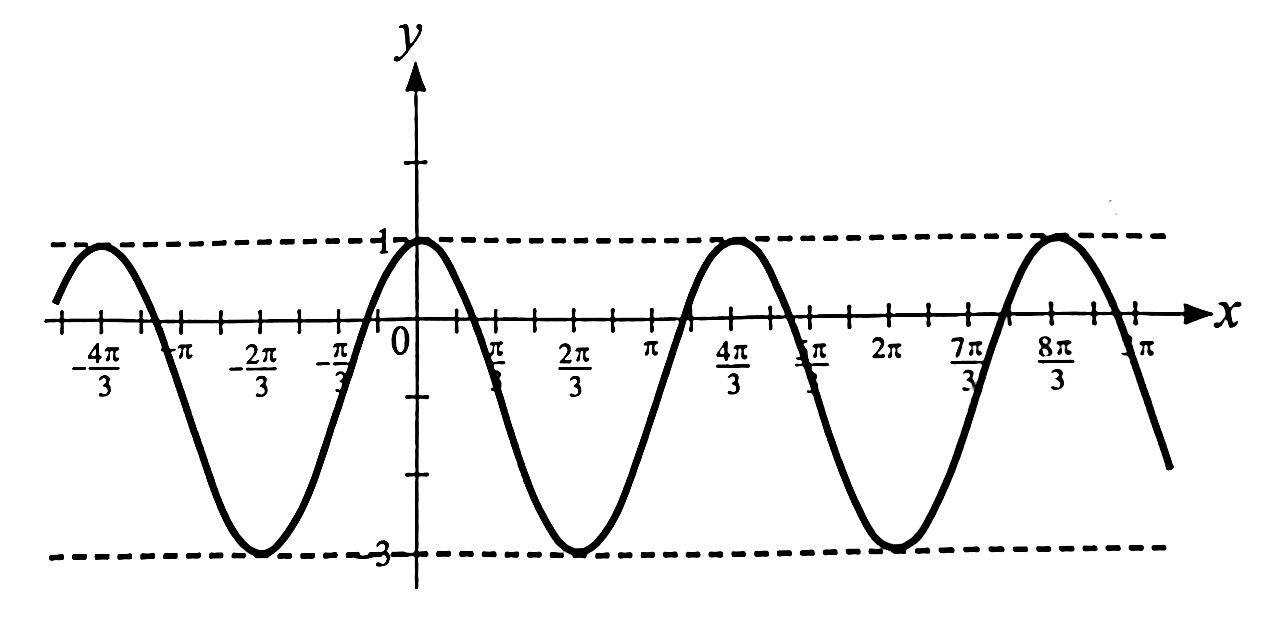
\includegraphics[width=0.55\textwidth]{assets/9-33.jpg}
            \end{center}

            \item Given that the function \( y=a \sin b x+c, a>0, b>0 \) has a maximum value of 4, a minimum value of -2, and the smallest positive period is \( \dfrac{\pi}{2} \), find the values of \( a, b, c \).
            
            \item The figure below shows the graph of \( I=I_m \sin \omega t \), representing the sinusoidal alternating current intensity, \( I \) (in amperes), as a function of time, \( t \) (in milliseconds), where \( I_m \) is the maximum current intensity, and \( \omega \) is the angular velocity of the rotating coil inside the generator. Find \( I_m \) and \( \omega \).
            \begin{center}
                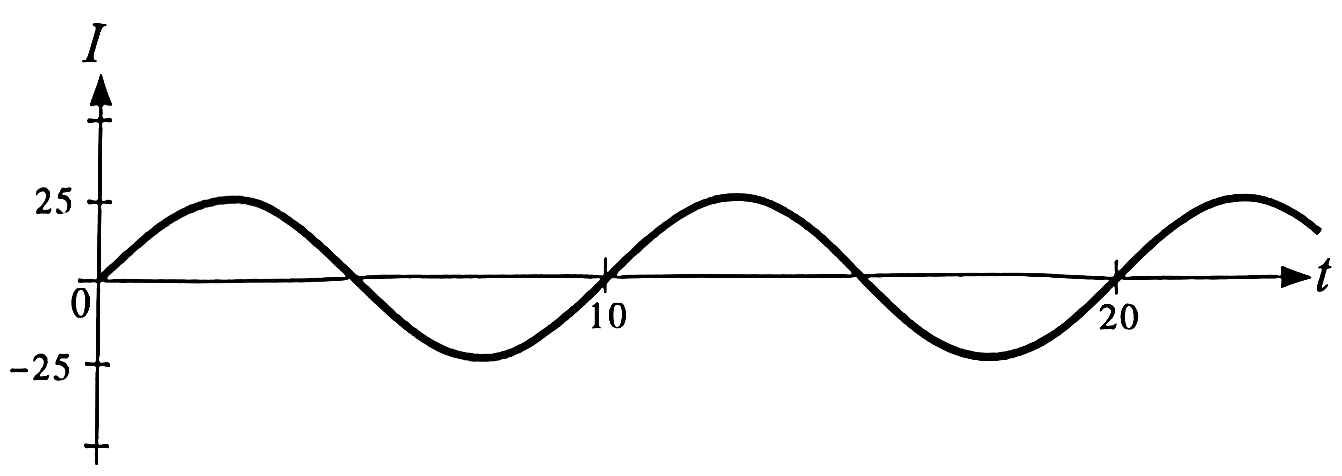
\includegraphics[width=0.55\textwidth]{assets/9-34.jpg}
            \end{center}

            \item Using computer software, plot the following functions in order in the same Cartesian coordinate system. Determine the periods of the following functions and explain how to obtain the plots of the following functions by transforming the plot of \( y=\tan x \):
            \begin{tasks}[label=(\alph*)](2)
                \task \( y=\tan \dfrac{x}{3} \)
                \task \( y=\tan \left(\dfrac{x}{3}-\dfrac{\pi}{4}\right) \)
                \task \( y=\tan \left(\dfrac{\pi}{4}-\dfrac{x}{3}\right) \)
                \task \( y=\dfrac{1}{2} \tan \left(\dfrac{\pi}{4}-\dfrac{x}{3}\right) \)
            \end{tasks}
        \end{enumerate}

        \section{Inverse Trigonometric Functions}

        We have previously learned about the definitions and properties of trigonometric functions of arbitrary angles, understanding their periodic nature and non-one-to-one behaviour. To find a specific angle given trigonometric function values, we need to introduce the concept of \textbf{inverse trigonometric functions}.

        \subsection*{Inverse Sine Function}
        \begin{center}
            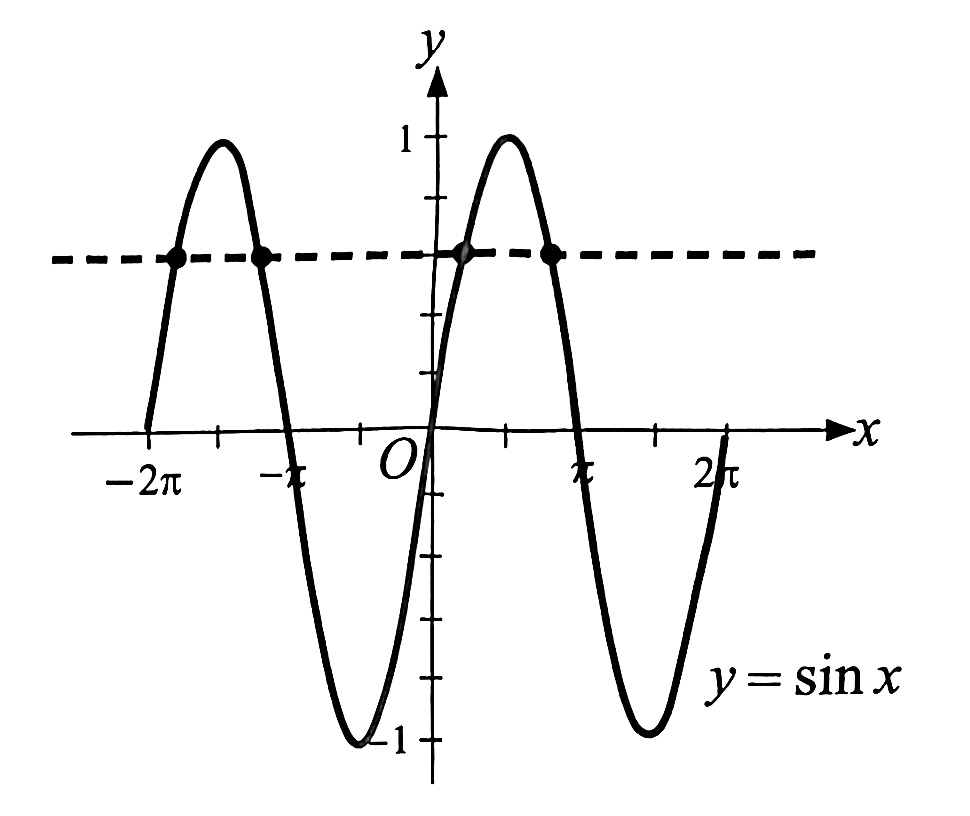
\includegraphics[width=0.4\textwidth]{assets/9-35.jpg}
        \end{center}

        The sine function \( y=\sin x \) is not one-to-one on \( \mathbb{R} \). However, we observe that \( y=\sin x \) is a one-to-one mapping on the interval \( \left[-\dfrac{\pi}{2}, \dfrac{\pi}{2}\right] \). Therefore, it has an inverse function (see the figure above).
        
        The inverse function of the function \( y=\sin x \) on the interval \( x \in\left[-\dfrac{\pi}{2}, \dfrac{\pi}{2}\right] \) is called the inverse sine function, generally denoted as:
        
        \begin{info}[Inverse Sine Function]
                
                \noindent $y=\sin^{-1} x \text{ or } y=\arcsin x $
                
                \noindent Domain is \( [-1,1] \) and range is \( \left[-\dfrac{\pi}{2}, \dfrac{\pi}{2}\right] \).
            \end{info}

    \begin{vwcol}[widths={0.6,0.4}, sep=0.5cm, rule=0pt]
        From the figure on the right, we can see that the graphs of \( y=\sin x \) for \( x \in\left[-\dfrac{\pi}{2}, \dfrac{\pi}{2}\right] \) and \( y=\sin^{-1} x \) are symmetric about the line \( y=x \). Furthermore, we can see that the graph of the inverse sine function is symmetric about the origin, i.e. \( \sin^{-1}(-x)=-\sin^{-1} x \) for \( x \in[-1,1] \).

        \noindent \parbox{0.6\textwidth}{\begin{warn}[Keep in Mind]
            
            \noindent The notation \( \sin^{-1} x \) does not mean \( \dfrac{1}{\sin x} \).
        \end{warn}}
        
        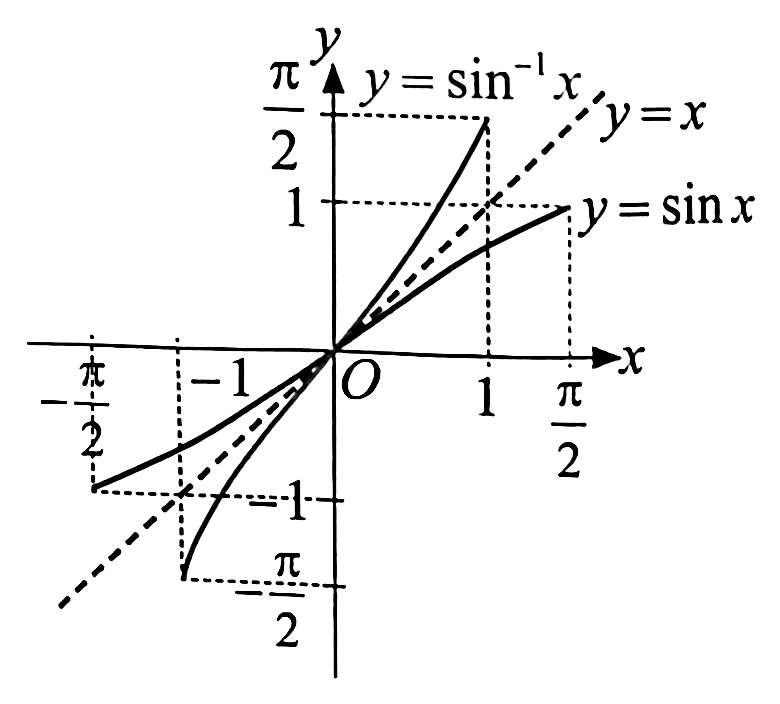
\includegraphics[width=0.3\textwidth]{assets/9-36.jpg}
\end{vwcol}

\newpage
\begin{question}
    Find the value of the following inverse sine functions:
    \begin{tasks}[label=(\alph*)](2)
        \task $\sin ^{-1} \dfrac{\sqrt{2}}{2}$
        \task $\sin ^{-1}(-0.1)$
    \end{tasks}

    \sol{}
    \vspace{-1em}
    \begin{enumerate}[label=(\alph*)]
        \item $\begin{aligned}[t] & \because \text{In the interval }\left[-\dfrac{\pi}{2}, \dfrac{\pi}{2}\right]\text{, } \sin \dfrac{\pi}{4}=\dfrac{\sqrt{2}}{2} \text {, } \\ & \therefore \sin ^{-1} \dfrac{\sqrt{2}}{2}=\dfrac{\pi}{4}\end{aligned}$
        \item $\sin ^{-1}(-0.1)=-5^{\circ} 44'$
    \end{enumerate}
\end{question}
\vspace{-2em}
\practice{9.4a}
Without using a calculator, complete the following table:
\begin{center}
    \begin{tblr}{|c|c|c|c|c|c|c|c|c|c|}
        \hline$x$ & $-1$ & $-\dfrac{\sqrt{3}}{2}$ & $-\dfrac{\sqrt{2}}{2}$ & $-\dfrac{1}{2}$ & $0$ & $\dfrac{1}{2}$ & $\dfrac{\sqrt{2}}{2}$ & $\dfrac{\sqrt{3}}{2}$ & $1$ \\
        \hline $\sin ^{-1} x$ & & & & & & & & & \\
        \hline
        \end{tblr}
\end{center}

\subsection*{Inverse Cosine Function}
\vspace{-1em}
\begin{center}
    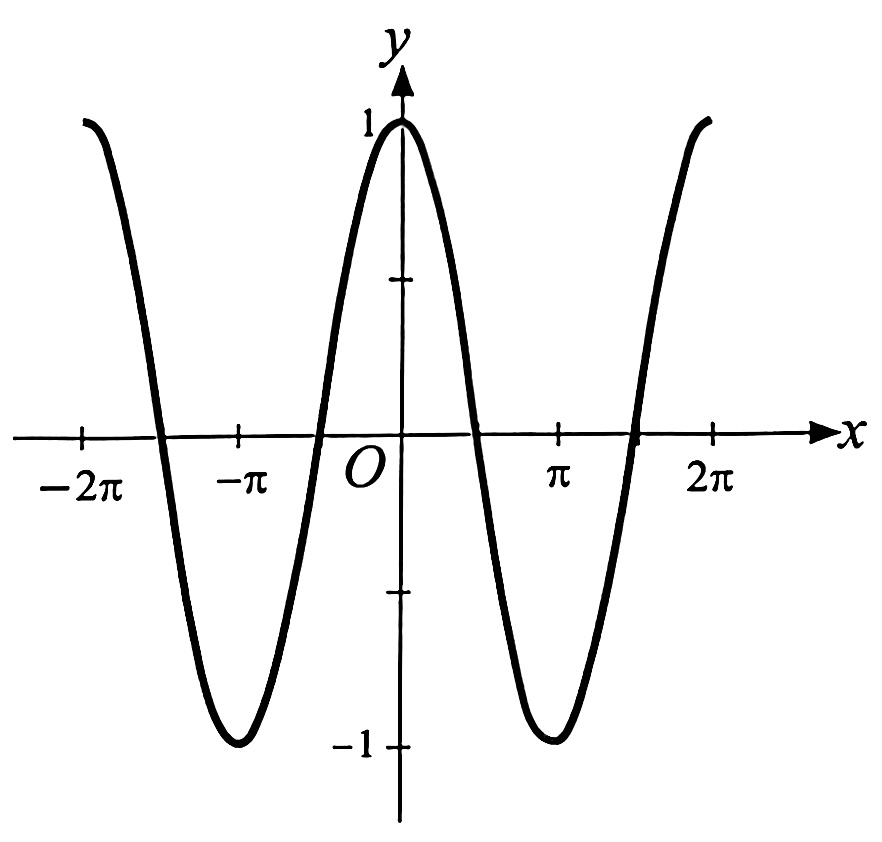
\includegraphics[width=0.35\textwidth]{assets/9-37.jpg}
\end{center}
\vspace{-1em}
We use the same approach to study the \textbf{inverse cosine function}.

As shown in the figure above, the function \( y=\cos x \) is a one-to-one mapping on the interval \( [0, \pi] \), so it has an inverse function. The inverse cosine function is denoted as
\begin{info}[Inverse Cosine Function]
    
    \noindent $y=\cos^{-1} x \text{ or } y=\arccos x $
    
    \noindent Domain is \( [-1,1] \) and range is \( [0, \pi] \).
\end{info}

The graph of the inverse cosine function \( y=\cos^{-1} x \) is shown in the figure below. It is symmetric about the line \( y=x \) with respect to the graph of the cosine function \( y=\cos x \) on the interval \( [0, \pi] \).
\begin{center}
    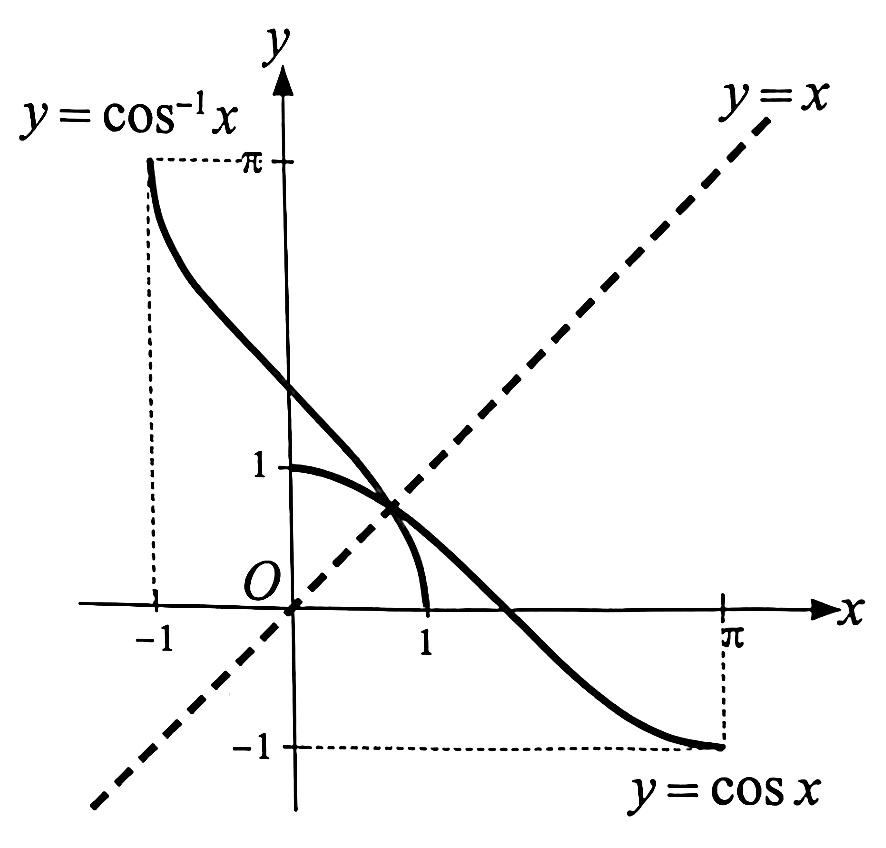
\includegraphics[width=0.35\textwidth]{assets/9-38.jpg}
\end{center}
\begin{question}
    Find the value of the following inverse cosine functions:
    \begin{tasks}[label=(\alph*)](2)
        \task $\cos ^{-1} \dfrac{\sqrt{2}}{2}$
        \task $\cos ^{-1}\left(-\dfrac{\sqrt{2}}{2}\right)$
    \end{tasks}

    \sol{}
    \vspace{-1em}
    \begin{enumerate}[label=(\alph*)]
        \item $\begin{aligned}[t] & \because \text { In the interval }[0, \pi] \text {, } \cos \dfrac{\pi}{4}=\dfrac{\sqrt{2}}{2} \text {, } \\ & \therefore \cos ^{-1} \dfrac{\sqrt{2}}{2}=\dfrac{\pi}{4}\end{aligned}$
        \item $\begin{aligned}[t] & \because \text { In the interval }[0, \pi] \text {, } \cos \dfrac{3 \pi}{4}=-\dfrac{\sqrt{2}}{2} \text {, } \\ & \therefore \cos ^{-1}\left(-\dfrac{\sqrt{2}}{2}\right)=\dfrac{3 \pi}{4} \text { 。 }\end{aligned}$
    \end{enumerate}
\end{question}
\practice{9.4b}
Without using a calculator, complete the following table:
\begin{center}
    \begin{tblr}{|c|c|c|c|c|c|c|c|c|c|c|c|}
        \hline$x$ & $-1$ & $-\dfrac{\sqrt{3}}{2}$ & $-\dfrac{\sqrt{2}}{2}$ & $-\dfrac{1}{2}$ & $0$ & $\dfrac{1}{2}$ & $\dfrac{\sqrt{2}}{2}$ & $\dfrac{\sqrt{3}}{2}$ & $1$\\
        \hline $\cos ^{-1} x$ & & & & & & & & & \\
        \hline
        \end{tblr}
\end{center}

\newpage
\subsection*{Inverse Tangent Function}
\begin{center}
    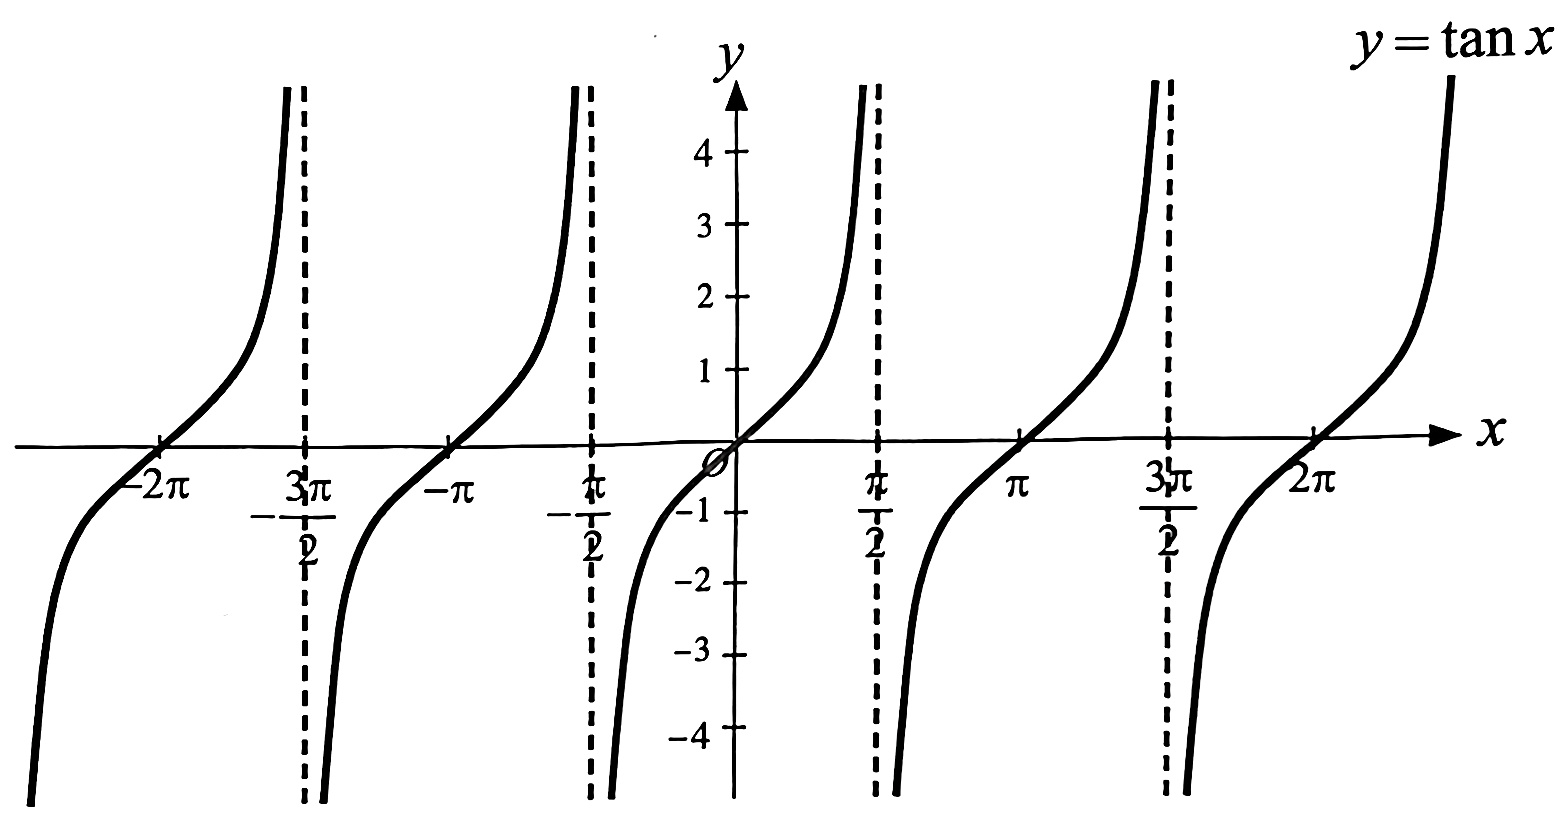
\includegraphics[width=0.6\textwidth]{assets/9-39.jpg}
\end{center}
The tangent function \( y=\tan x \) is a one-to-one mapping on \( \left(-\dfrac{\pi}{2}, \dfrac{\pi}{2}\right) \). Its inverse function is called the \textbf{inverse tangent function}, denoted as
\begin{info}[Inverse Tangent Function]
    
    \noindent $y=\tan^{-1} x \text{ or } y=\arctan x $
    
    \noindent Domain is \( (-\infty, \infty) \) and range is \( \left(-\dfrac{\pi}{2}, \dfrac{\pi}{2}\right) \).
\end{info}

As shown in the figure below, the graph of the inverse tangent function \( y=\tan^{-1} x \) is symmetric about the line \( y=x \) with respect to the graph of the tangent function \( y=\tan x \) on the interval \( x \in\left(-\dfrac{\pi}{2}, \dfrac{\pi}{2}\right) \). Furthermore, the graph of the inverse tangent function is symmetric about the origin, i.e. \( \tan^{-1}(-x)=-\tan^{-1} x \) for \( x \in \mathbb{R} \).
\begin{center}
    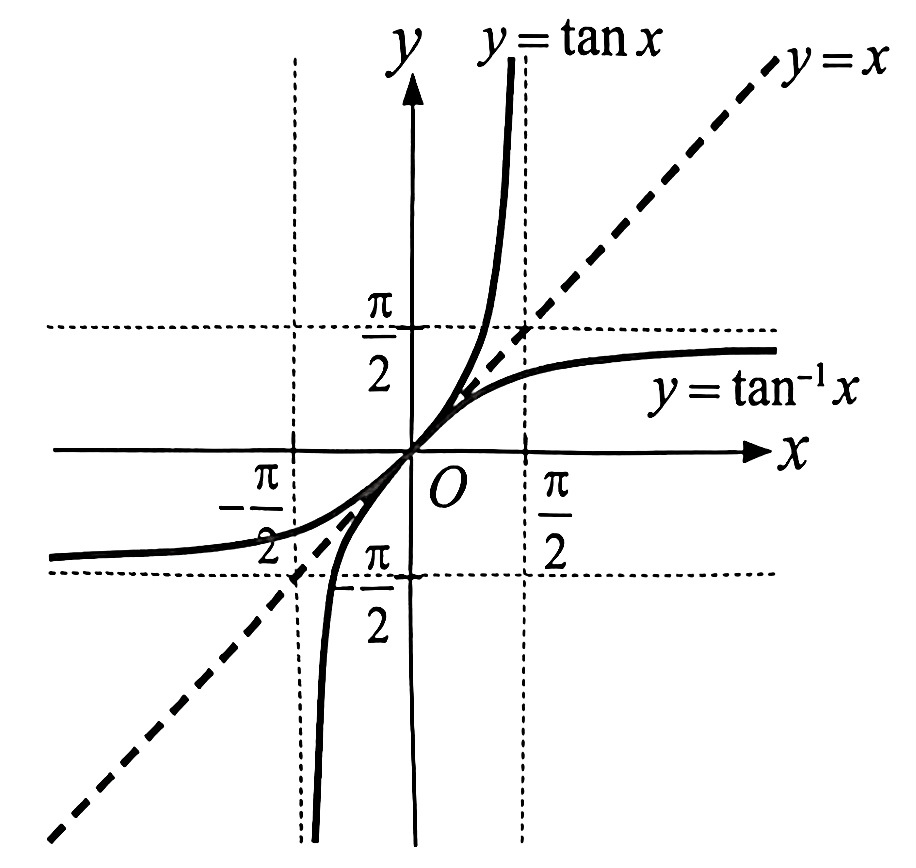
\includegraphics[width=0.35\textwidth]{assets/9-40.jpg}
\end{center}
\begin{question}
    Find the value of the following inverse tangent functions:
    \begin{tasks}[label=(\alph*)](2)
        \task $\tan ^{-1} 0$
        \task $\tan ^{-1}(-2)$
    \end{tasks}

    \sol{}
    \vspace{-1em}
    \begin{tasks}[label=(\alph*)](2)
        \task $\tan ^{-1} 0=0$
        \task $\tan ^{-1}(-2)=-1.107$
    \end{tasks}
\end{question}
\practice{9.4c}
Without using a calculator, complete the following table:
\begin{center}
    \begin{tblr}{|c|c|c|c|c|c|c|c|}
        \hline$x$ & $-\sqrt{3}$ & $-1$ & $-\dfrac{1}{\sqrt{3}}$ & $0$ & $\dfrac{1}{\sqrt{3}}$ & $1$ & $\sqrt{3}$ \\
        \hline $\tan ^{-1} x$ & & & & & & & \\
        \hline
        \end{tblr}
\end{center}

The properties of these inverse trigonometric functions are summarized in the table below:
\begin{center}
    \begin{tblr}{|c|c|c|c|}
        \hline Functions & $y=\sin ^{-1} x$ & $y=\cos ^{-1} x$ & $y=\tan ^{-1} x$ \\
        \hline Graphs & 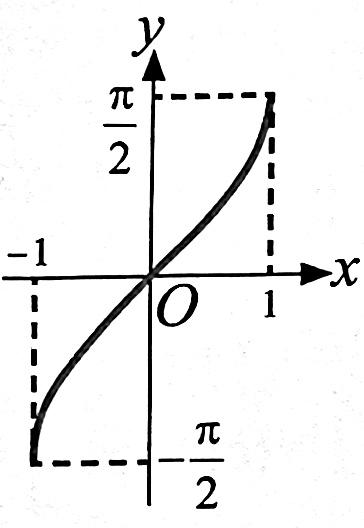
\includegraphics[width=0.13\textwidth]{assets/9-41.jpg} & 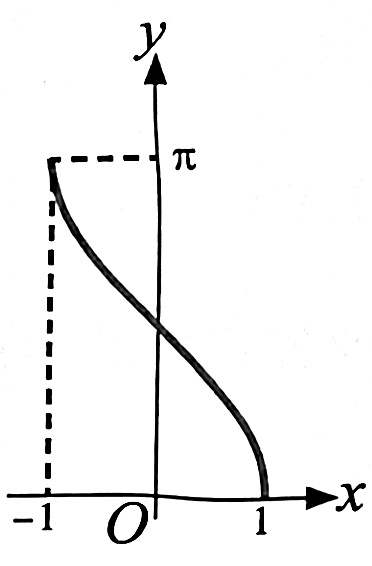
\includegraphics[width=0.13\textwidth]{assets/9-42.jpg} & 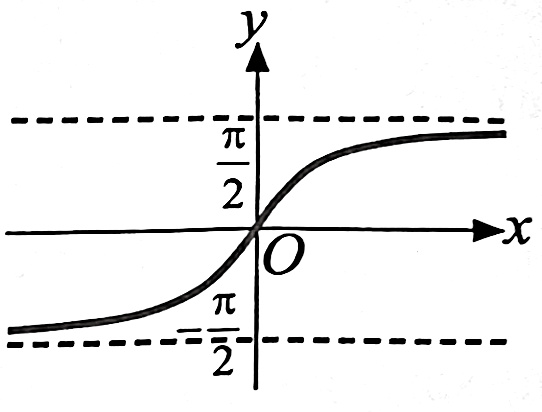
\includegraphics[width=0.2\textwidth]{assets/9-43.jpg} \\
        \hline Domains & {$[-1,1]$} & {$[-1,1]$} & $\mathbb{R}$ \\
        \hline Ranges & {$\left[-\dfrac{\pi}{2}, \dfrac{\pi}{2}\right]$} & {$[0, \pi]$} & $\left(-\dfrac{\pi}{2}, \dfrac{\pi}{2}\right)$ \\
        \hline
        \end{tblr}
\end{center}
\begin{question}
    Express the angle \( x \) in the form of inverse trigonometric functions for \( \cos x=-\dfrac{4}{5} \) where \( \pi < x < 2 \pi \).

    \sol{}
    \begin{flalign*}
        & \because \cos \left(\cos ^{-1} \dfrac{4}{5}\right)=\dfrac{4}{5} \text { and } \cos ^{-1} \dfrac{4}{5} \in\left(0, \dfrac{\pi}{2}\right),\ \therefore x=\pi+\cos ^{-1} \dfrac{4}{5}&
    \end{flalign*}
\end{question}
\vspace{-2em}
\exercise{9.4}
\begin{enumerate}
    \item Given a right triangle \(ABC\) where the adjacent side \(AB\) is 5 and the hypotenuse \(AC\) is 7, express angle \(A\) using inverse trigonometric functions.
    
    \item Determine whether the following expressions has meaning.
    \begin{tasks}(3)
        \task \( \sin^{-1} \dfrac{\pi}{3} \)
        \task \( \cos^{-1} \sqrt{2} \)
        \task \( \tan^{-1} \sqrt{3} \)
    \end{tasks}
    
    \item Express the angles in the following equations using inverse trigonometric functions:
    \begin{tasks}(3)
        \task \( \sin \dfrac{\pi}{3}=\dfrac{\sqrt{3}}{2} \)
        \task \( \sin \dfrac{2\pi}{3}=\dfrac{\sqrt{3}}{2} \)
        \task \( \cos \dfrac{3\pi}{4}=-\dfrac{\sqrt{2}}{2} \)
    \end{tasks}
    
    \item Find the values of the following expressions:
    \begin{tasks}(3)
        \task \( \sin^{-1} 0.6959 \)
        \task \( \cos^{-1}\left(-\dfrac{\pi}{8}\right) \)
        \task \( \tan^{-1}\left(\tan \dfrac{3\pi}{4}\right) \)
    \end{tasks}
\end{enumerate}

\revision{9}
\begin{enumerate}
    \item Given that the terminal point of angle \( \theta \) intersects a unit circle at \( \left(\dfrac{\sqrt{5}}{5},-\dfrac{2 \sqrt{5}}{5}\right) \), find the values of sine, cosine, and tangent of angle \( \theta \).
\end{enumerate}
    \begin{vwcol}[widths={0.7,0.3}, sep=0.5cm, rule=0pt]
        \parbox{0.7\textwidth}{
            \begin{enumerate}[start=2]
                \vspace*{-2.4em}
                \item Given that \( (-6, y) \) lies on the terminal side of angle \( \theta \), and \( \cos \theta=-\dfrac{4}{5} \), find the value of \( y \) and \( \tan \theta \).
        
                \item As shown in the diagram to the right, given \( \tan x^{\circ}=-\dfrac{2}{3} \) and \( QR=21 \mathrm{~cm} \), find \( SQ \).
            \end{enumerate}
        }
        
    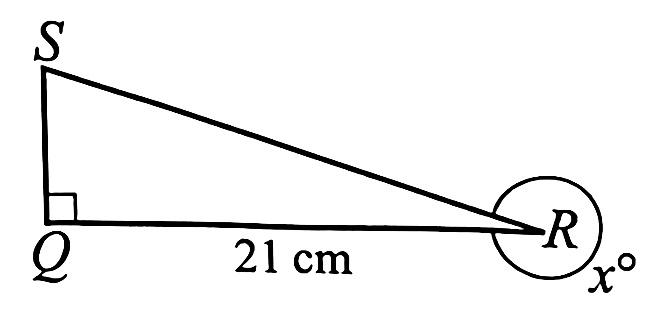
\includegraphics[width=0.25\textwidth]{assets/9-44.jpg}
    \end{vwcol}
    \vspace{-3.6em}
\begin{enumerate}[start=4]
    \item If \( \cos \theta=\dfrac{1}{4} \), without finding the angle \( \theta \), find the values of \( \sin \theta \) and \( \tan \theta \).
    \item Given that \( 4 \tan \theta=-3 \) and \( \cos \theta \) is negative, without finding the angle \( \theta \), find the value of \( \dfrac{5 \sin \theta+4 \sec \theta}{3 \cot \theta+10 \cos \theta} \).
    \item Given that \( \dfrac{13 \cos x+1}{2-4 \cos x}=3 \) and \( \tan x<0 \), without finding the angle \( x \), find the value of \( \sin x \).
    \item Let \( \cos 140^{\circ}=k \). Express the values of \( \tan 40^{\circ} \) and \( \sin 50^{\circ} \) in terms of \( k \).
    \item Find the values of the following expressions without using a calculator:
    \begin{enumerate}[label=(\alph*)]
        \item \( \sin 420^{\circ} \cos 750^{\circ}+\sin (-330^{\circ}) \cos (-660^{\circ}) \)
        \item \( 5 \sin 90^{\circ}+2 \cos 0^{\circ}-3 \sin 270^{\circ}+10 \cos 180^{\circ} \)
        \item \( \dfrac{\sin \dfrac{2 \pi}{3}-\cos \dfrac{4 \pi}{3}-\tan \dfrac{5 \pi}{3}}{\cos \dfrac{5 \pi}{6}+\tan \dfrac{5 \pi}{3}+\sin \dfrac{7 \pi}{6}} \)
        \item \( \tan (23^{\circ}+\theta) \tan (67^{\circ}-\theta) \)
        \item \( \dfrac{\sin ^2(\alpha+\pi) \cos (\pi+\alpha) \cot (\alpha-2 \pi)}{\tan (\pi+\alpha) \cos ^3(-\alpha-\pi)} \)
    \end{enumerate}
    
    \item Given that \( f(\theta)=\dfrac{2 \sin ^3 \theta+\cos ^2\left(\theta+\dfrac{\pi}{2}\right)+2 \sin (-\theta-\pi)}{2+2 \sin ^2 \theta-\sin (-\theta)} \), find the value of \( f\left(\dfrac{2030 \pi}{3}\right) \) without using a calculator.
    
    \item Given that \( A, B, C \) are the interior angles of a triangle, prove \( \tan \dfrac{A+C}{4}=-\tan \dfrac{3 \pi+B}{4} \).
    
    \item If \( \dfrac{\operatorname{cosec}^2(2 \pi-\theta)}{\sec^2(\pi+\theta)}=3 \) and \( -\dfrac{\pi}{2}<\theta<0 \), without finding the angle \( \theta \), find the value of \( \sin \theta \).
    
    \item Given \( \dfrac{\pi}{10}<\theta<\dfrac{3 \pi}{5} \) and \( \cos \left(\theta+\dfrac{2 \pi}{5}\right)=p \), express \( \cos \left(\dfrac{3 \pi}{5}-\theta\right) \) in terms of \( p \).
    
    \item Plot the following functions in order in the same Cartesian coordinate system on the interval \( 0 \leq x \leq 4 \pi \). Hence, find their ranges:
    \begin{tasks}[label=(\alph*)](2)
        \task \( y=\cos 2 x \)
        \task \( y=\cos \left(2 x+\dfrac{\pi}{3}\right) \)
        \task \( y=2 \cos \left(2 x+\dfrac{\pi}{3}\right) \)
        \task \( y=\left|2 \cos \left(2 x+\dfrac{\pi}{3}\right)\right| \)
    \end{tasks}
    
    \item Plot the function \( y=\cos^{-1} x-\dfrac{\pi}{2} \). Hence, find its domain and range.
    
    \item Given an isosceles triangle with the base equal to \(\dfrac{9}{5}\) times the height, express the base angle of this triangle using inverse trigonometric functions.
    
    \item \parbox[t]{\textwidth}{\begin{center}
        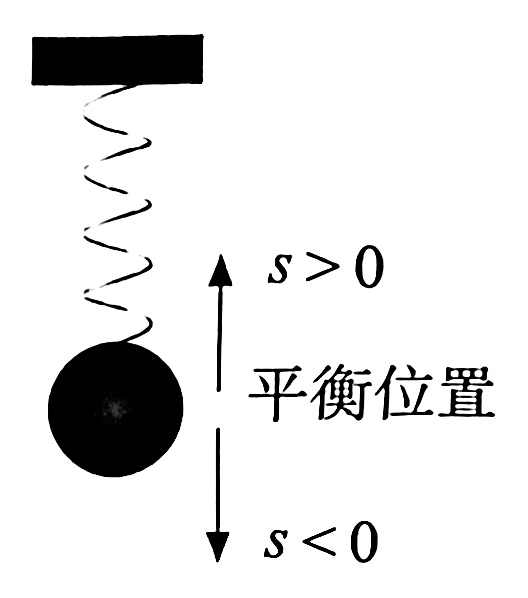
\includegraphics[width=0.2\textwidth]{assets/9-45.jpg}
    \end{center}}
    
    A ball hanging on a spring oscillates up and down. The distance \( s \), in centimetres, from the equilibrium position at time \( t \) seconds is defined by \( s=2 \sin \left(t+\dfrac{\pi}{4}\right) \).
    \begin{enumerate}
        \item Sketch a simple graph of this function for \( 0 \leq t \leq 4 \pi \).
        \item Find:
        \begin{enumerate}
            \item The initial position of the ball;
            \item The highest and lowest positions of the ball;
            \item The time required for the ball to complete one oscillation.
        \end{enumerate}
    \end{enumerate}
    
    \item The figure below shows the measured tidal heights \( y \) in meters at Pulau Langkawi from the early morning of July 31st to the early morning of August 2nd.
    \begin{center}
        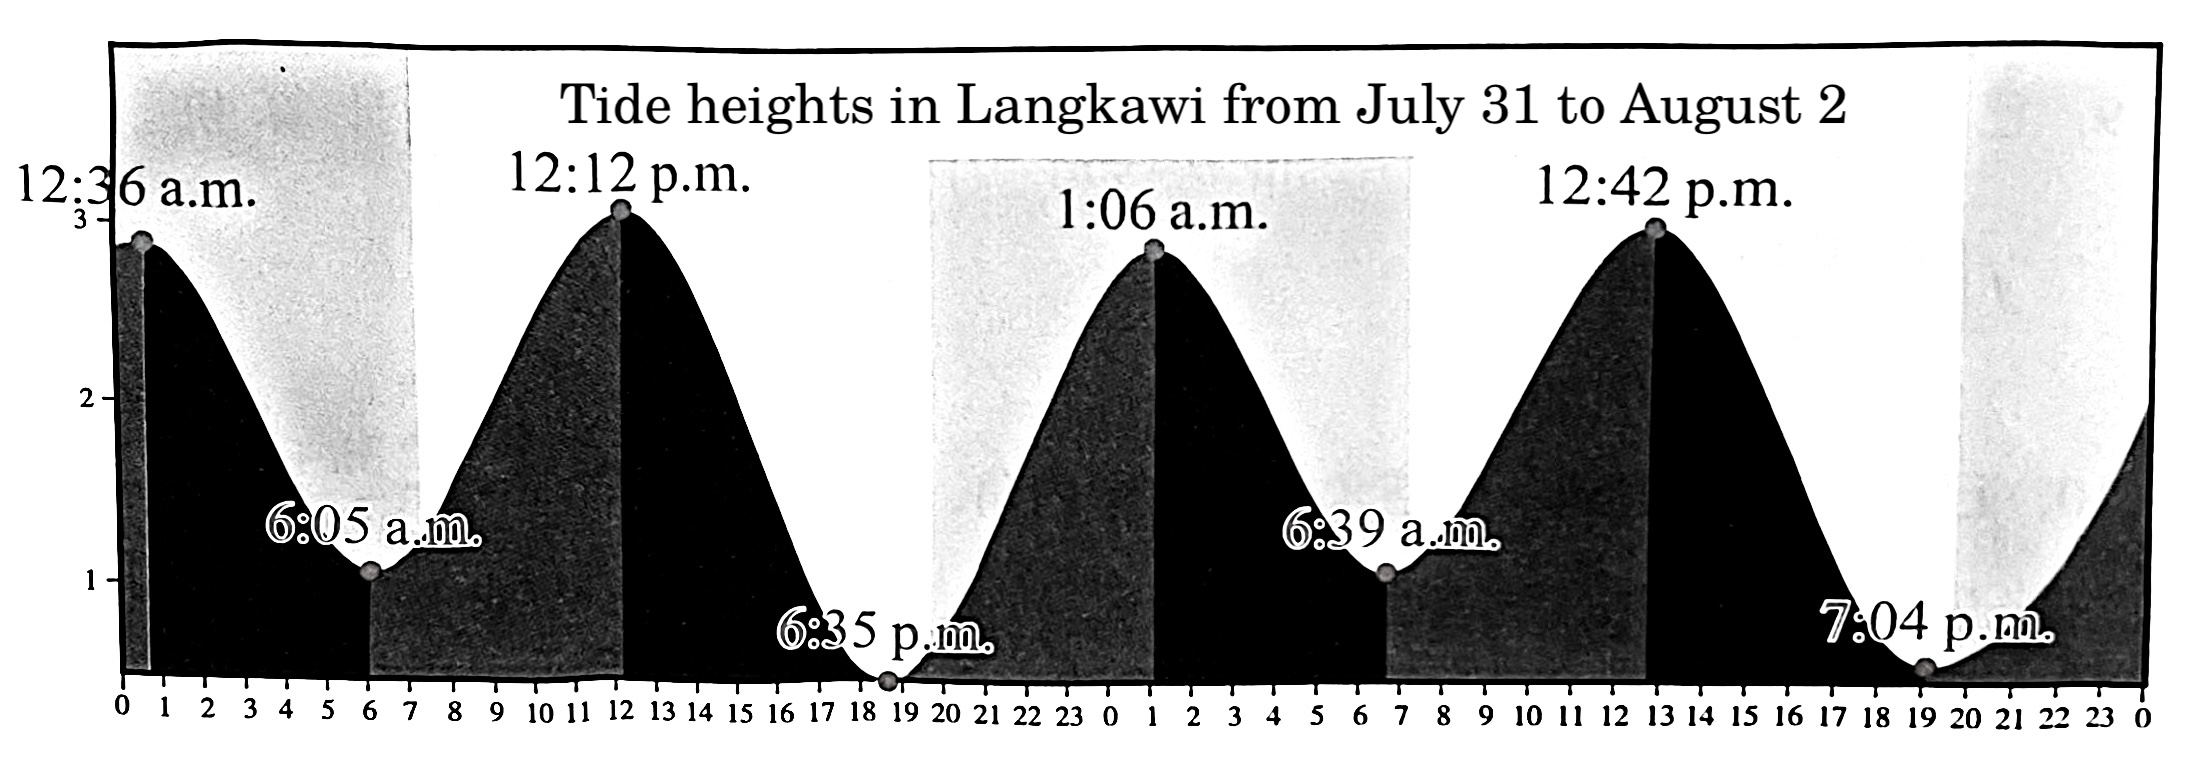
\includegraphics[width=0.7\textwidth]{assets/9-46.jpg}
    \end{center}

    The above curve can be approximated as the graph of the cosine function \( y = a \sin (b x + c) + d, a > 0, b > 0 \).
    \begin{enumerate}[label=(\alph*)]
        \item Base on the figure above, find the expression of the function $y=a \sin (b x+c)+d$.
        \item If a class of students wants to conduct learning activities on the beach when the tide recedes on August 4th, which period is most suitable? Give your reasons.
    \end{enumerate}
\end{enumerate}
\end{document}